\titleformat{\chapter}[display]
  {\normalfont\Large\bfseries}{\centering Tuần 5}{10pt}{\centering\Huge\bfseries}
  
\chapter{Dao Động}

Trong phần này, chúng ta sẽ tìm hiểu về chuyển động dao động. Bắt đầu từ những thứ cơ bản nhất như con lắc đơn, đến những hệ phức tạp như dao động liên kết giữa các vật. 




\section{Dao động hệ 1 chất điểm}
\subsection{Dao động điều hoà}
Đầu tiên chúng ta xem xét hệ cơ bản nhất của dao động. Chỉ bao gồm duy nhất 1 chất điểm có khối lượng \(m\). Trong quá trình chuyển động của chất điểm, nó phải chịu một lực có dạng \(F = - k x\). Lực này có đặc điểm luôn hướng về vị trí có \(x = 0\). 

\begin{figure}[!htb]
    \centering
    \begin{frame}{Số phức}
    \begin{center}
        \begin{minipage}{0.4\linewidth}
            \resizebox{1\linewidth}{!}{


\tikzset{every picture/.style={line width=0.75pt}} %set default line width to 0.75pt        

\begin{tikzpicture}[x=0.75pt,y=0.75pt,yscale=-1,xscale=1]
%uncomment if require: \path (0,15225); %set diagram left start at 0, and has height of 15225

%Straight Lines [id:da5015611160293443] 
\draw    (526,6086) -- (683.5,6086) ;
\draw [shift={(685.5,6086)}, rotate = 180] [color={rgb, 255:red, 0; green, 0; blue, 0 }  ][line width=0.75]    (10.93,-3.29) .. controls (6.95,-1.4) and (3.31,-0.3) .. (0,0) .. controls (3.31,0.3) and (6.95,1.4) .. (10.93,3.29)   ;
%Straight Lines [id:da7739785169188371] 
\draw    (526,6086) -- (526,5966) ;
\draw [shift={(526,5964)}, rotate = 90] [color={rgb, 255:red, 0; green, 0; blue, 0 }  ][line width=0.75]    (10.93,-3.29) .. controls (6.95,-1.4) and (3.31,-0.3) .. (0,0) .. controls (3.31,0.3) and (6.95,1.4) .. (10.93,3.29)   ;
%Straight Lines [id:da38078718023855684] 
\draw  [dash pattern={on 0.84pt off 2.51pt}]  (526,6033) -- (608.5,6033) ;
\draw [shift={(608.5,6033)}, rotate = 0] [color={rgb, 255:red, 0; green, 0; blue, 0 }  ][fill={rgb, 255:red, 0; green, 0; blue, 0 }  ][line width=0.75]      (0, 0) circle [x radius= 3.35, y radius= 3.35]   ;
%Straight Lines [id:da36972469805515473] 
\draw  [dash pattern={on 0.84pt off 2.51pt}]  (608.5,6033) -- (608.5,6086) ;

% Text Node
\draw (474,5948) node [anchor=north west][inner sep=0.75pt]    {$Im( z)$};
% Text Node
\draw (615,6008) node [anchor=north west][inner sep=0.75pt]    {$z\ =\ a\ +\ ib$};
% Text Node
\draw (682,6092) node [anchor=north west][inner sep=0.75pt]    {$Re( z)$};
% Text Node
\draw (601,6091) node [anchor=north west][inner sep=0.75pt]    {$a$};
% Text Node
\draw (505,6022) node [anchor=north west][inner sep=0.75pt]    {$b$};
% Text Node
\draw (507,6083) node [anchor=north west][inner sep=0.75pt]    {$O$};


\end{tikzpicture}}
        \end{minipage}
        \hspace{2mm}
        \begin{minipage}{0.4\linewidth}
            Số ảo \(\mathbf{i}\) được định nghĩa \cite{gilbert2009introduction}
            \begin{equation}
                i = \sqrt{-1}.
                \label{eq:1.1_1}
            \end{equation}
            Không gian số phức là 
            \begin{equation*}
                \mathcal{C} = (a,b) | a,b \in \mathcal{R}
            \end{equation*}
        \end{minipage}
    \end{center}
\end{frame}

\begin{frame}{Công thức euler}
    \begin{mdframed}[backgroundcolor=BlueDefault!10, linecolor=BlueDefault, linewidth=0.5pt, roundcorner=1pt]
        Công thức euler gọi là phép quay một góc \(\theta\) trong mặt phẳng phức.
        \begin{equation}
            e^{i\theta} = \cos{\theta} + i \sin{\theta}
            \label{eq:1.1_2}
        \end{equation}
    \end{mdframed}
    \vspace{2mm}
    
    Ví dụ: áp dụng phép quay \(\theta\) cho số phức \(z = a + i b\)
    \begin{center}
        \begin{minipage}{0.4\linewidth}
            \begin{equation*}
            \begin{split}
                \left[
            \begin{array}{c}
                a' \\
                b'
            \end{array}
            \right]  &= \left[\begin{array}{cc}
               \cos{\theta}  & -\sin{\theta} \\
               \sin{\theta}  & \cos{\theta}
            \end{array} \right] \left[
            \begin{array}{c}
                a \\
                b
            \end{array}
            \right]  \\
           z' &=  e^{i\theta}z
            \end{split}
            \end{equation*}
        \end{minipage}
        \hspace{1mm}
        \begin{minipage}{0.4\linewidth}
            \begin{center}
                \resizebox{1\linewidth}{!}{


\tikzset{every picture/.style={line width=0.75pt}} %set default line width to 0.75pt        

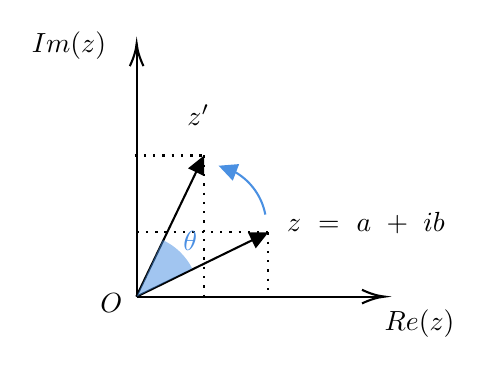
\begin{tikzpicture}[x=0.75pt,y=0.75pt,yscale=-1,xscale=1]
%uncomment if require: \path (0,15225); %set diagram left start at 0, and has height of 15225

%Straight Lines [id:da5015611160293443] 
\draw    (526,6086) -- (643.5,6086) ;
\draw [shift={(645.5,6086)}, rotate = 180] [color={rgb, 255:red, 0; green, 0; blue, 0 }  ][line width=0.75]    (10.93,-3.29) .. controls (6.95,-1.4) and (3.31,-0.3) .. (0,0) .. controls (3.31,0.3) and (6.95,1.4) .. (10.93,3.29)   ;
%Straight Lines [id:da7739785169188371] 
\draw    (526,6086) -- (526,5966) ;
\draw [shift={(526,5964)}, rotate = 90] [color={rgb, 255:red, 0; green, 0; blue, 0 }  ][line width=0.75]    (10.93,-3.29) .. controls (6.95,-1.4) and (3.31,-0.3) .. (0,0) .. controls (3.31,0.3) and (6.95,1.4) .. (10.93,3.29)   ;
%Straight Lines [id:da6097015977657645] 
\draw  [dash pattern={on 0.84pt off 2.51pt}]  (526,6055) -- (589.5,6055) ;
%Straight Lines [id:da06830863122513897] 
\draw  [dash pattern={on 0.84pt off 2.51pt}]  (589.5,6055) -- (589.5,6086) ;
%Straight Lines [id:da1339436079722769] 
\draw    (526,6086) -- (586.8,6056.32) ;
\draw [shift={(589.5,6055)}, rotate = 153.98] [fill={rgb, 255:red, 0; green, 0; blue, 0 }  ][line width=0.08]  [draw opacity=0] (8.93,-4.29) -- (0,0) -- (8.93,4.29) -- cycle    ;
%Straight Lines [id:da12876867450395124] 
\draw    (525.83,6086) -- (557.2,6020.7) ;
\draw [shift={(558.5,6018)}, rotate = 115.66] [fill={rgb, 255:red, 0; green, 0; blue, 0 }  ][line width=0.08]  [draw opacity=0] (8.93,-4.29) -- (0,0) -- (8.93,4.29) -- cycle    ;
%Straight Lines [id:da6964942743081263] 
\draw  [dash pattern={on 0.84pt off 2.51pt}]  (525,6018) -- (558.5,6018) ;
%Straight Lines [id:da21207065554446136] 
\draw  [dash pattern={on 0.84pt off 2.51pt}]  (558.5,6018) -- (558.5,6086) ;
%Straight Lines [id:da7448312272789616] 
\draw [color={rgb, 255:red, 74; green, 144; blue, 226 }  ,draw opacity=1 ]   (573.49,6026.01) -- (568.31,6024.02) ;
\draw [shift={(565.51,6022.94)}, rotate = 21.06] [fill={rgb, 255:red, 74; green, 144; blue, 226 }  ,fill opacity=1 ][line width=0.08]  [draw opacity=0] (8.93,-4.29) -- (0,0) -- (8.93,4.29) -- cycle    ;
%Shape: Arc [id:dp7227532122430883] 
\draw  [draw opacity=0] (573.49,6026.01) .. controls (580.94,6030.31) and (586.36,6037.72) .. (587.99,6046.47) -- (558.5,6052) -- cycle ; \draw  [color={rgb, 255:red, 74; green, 144; blue, 226 }  ,draw opacity=1 ] (573.49,6026.01) .. controls (580.94,6030.31) and (586.36,6037.72) .. (587.99,6046.47) ;  
%Shape: Arc [id:dp5675882433264926] 
\draw  [draw opacity=0][fill={rgb, 255:red, 74; green, 144; blue, 226 }  ,fill opacity=0.52 ] (538.61,6058.77) .. controls (544.71,6061.6) and (549.7,6066.42) .. (552.75,6072.4) -- (526,6086) -- cycle ; \draw  [draw opacity=0] (538.61,6058.77) .. controls (544.71,6061.6) and (549.7,6066.42) .. (552.75,6072.4) ;  

% Text Node
\draw (474,5957) node [anchor=north west][inner sep=0.75pt]    {$Im( z)$};
% Text Node
\draw (597,6044) node [anchor=north west][inner sep=0.75pt]    {$z\ =\ a\ +\ ib$};
% Text Node
\draw (644,6091) node [anchor=north west][inner sep=0.75pt]    {$Re( z)$};
% Text Node
\draw (507,6083) node [anchor=north west][inner sep=0.75pt]    {$O$};
% Text Node
\draw (549,5992) node [anchor=north west][inner sep=0.75pt]    {$z'$};
% Text Node
\draw (547,6053) node [anchor=north west][inner sep=0.75pt]    {$\textcolor[rgb]{0.29,0.56,0.89}{\theta }$};


\end{tikzpicture}}
            \end{center}
        \end{minipage}
    \end{center}
\end{frame}
\begin{frame}{Số phức}
    \begin{mdframed}[backgroundcolor=BlueDefault!10, linecolor=BlueDefault, linewidth=0.5pt, roundcorner=1pt]
        Công thức euler còn là cách biểu diễn khác của số phức.
        \begin{equation}
            z = |z| e^{i\theta} = |z|(\cos{\theta} + i \sin{\theta})
            \label{eq:1.1_3}
        \end{equation}
        Với \(|z|\) là module của số phức \(z\), \(\theta\) là góc lệch của so với trục thực.
    \end{mdframed}
    \begin{center}
        \begin{minipage}{0.4\linewidth}
        \resizebox{1\linewidth}{!}{


\tikzset{every picture/.style={line width=0.75pt}} %set default line width to 0.75pt        

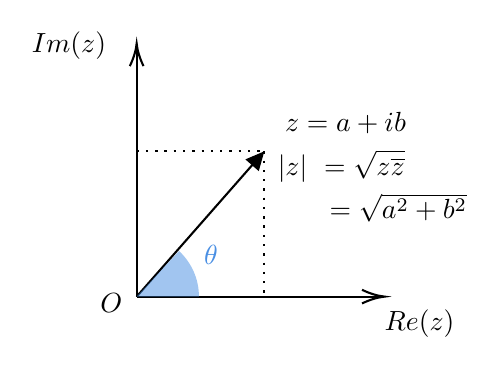
\begin{tikzpicture}[x=0.75pt,y=0.75pt,yscale=-1,xscale=1]
%uncomment if require: \path (0,15225); %set diagram left start at 0, and has height of 15225

%Straight Lines [id:da5597477618794069] 
\draw    (843,6091) -- (960.5,6091) ;
\draw [shift={(962.5,6091)}, rotate = 180] [color={rgb, 255:red, 0; green, 0; blue, 0 }  ][line width=0.75]    (10.93,-3.29) .. controls (6.95,-1.4) and (3.31,-0.3) .. (0,0) .. controls (3.31,0.3) and (6.95,1.4) .. (10.93,3.29)   ;
%Straight Lines [id:da12681955407125622] 
\draw    (843,6091) -- (843,5971) ;
\draw [shift={(843,5969)}, rotate = 90] [color={rgb, 255:red, 0; green, 0; blue, 0 }  ][line width=0.75]    (10.93,-3.29) .. controls (6.95,-1.4) and (3.31,-0.3) .. (0,0) .. controls (3.31,0.3) and (6.95,1.4) .. (10.93,3.29)   ;
%Straight Lines [id:da8100573273316289] 
\draw  [dash pattern={on 0.84pt off 2.51pt}]  (843,6021) -- (904.5,6021) ;
%Straight Lines [id:da18835817233889307] 
\draw  [dash pattern={on 0.84pt off 2.51pt}]  (904.5,6021) -- (904.5,6091) ;
%Straight Lines [id:da16390059449403382] 
\draw    (843,6091) -- (902.52,6023.25) ;
\draw [shift={(904.5,6021)}, rotate = 131.3] [fill={rgb, 255:red, 0; green, 0; blue, 0 }  ][line width=0.08]  [draw opacity=0] (8.93,-4.29) -- (0,0) -- (8.93,4.29) -- cycle    ;
%Shape: Arc [id:dp60111373870411] 
\draw  [draw opacity=0][fill={rgb, 255:red, 74; green, 144; blue, 226 }  ,fill opacity=0.52 ] (863.41,6069.02) .. controls (869.31,6074.49) and (873,6082.32) .. (873,6091) -- (843,6091) -- cycle ; \draw  [draw opacity=0] (863.41,6069.02) .. controls (869.31,6074.49) and (873,6082.32) .. (873,6091) ;  

% Text Node
\draw (791,5962) node [anchor=north west][inner sep=0.75pt]    {$Im( z)$};
% Text Node
\draw (913,6001) node [anchor=north west][inner sep=0.75pt]    {$z = a + ib$};
% Text Node
\draw (961,6096) node [anchor=north west][inner sep=0.75pt]    {$Re( z)$};
% Text Node
\draw (824,6088) node [anchor=north west][inner sep=0.75pt]    {$O$};
% Text Node
\draw (909.5,6019) node [anchor=north west][inner sep=0.75pt]    {$|z|\ =\sqrt{z \overline{z}}  $};
\draw (934.5,6040) node [anchor=north west][inner sep=0.75pt]    {$= \sqrt{a^2 + b^2} $};
% Text Node
\draw (874,6065) node [anchor=north west][inner sep=0.75pt]    {$\textcolor[rgb]{0.29,0.56,0.89}{\theta }$};


\end{tikzpicture}}
        \end{minipage}
        \hspace{3mm}
        \begin{minipage}{0.35\linewidth}
        Liên hợp phức: 
        \begin{equation}
            z = a + ib \rightarrow \overline{z} = a - ib.
            \label{eq:1.1_4}
        \end{equation}
        \end{minipage}
    \end{center}
\end{frame}
    \caption{}
    \label{fig:1.1}
\end{figure}

Ta sẽ dễ dàng viết được phương trình vi phân chuyển động (Hay nói cách khác chính là phương trình định luật II Newton).
\begin{equation}
    m \ddot{x} = -kx.
    \label{eq:1.1}
\end{equation}
Từ các phương pháp giải phương trình vi phân, ta có thể thu được nghiệm của phương trình trên.
\begin{equation}
    x = A \cos{ \left(\omega t + \varphi \right)}.
    \label{eq:1.2}
\end{equation}
Với \(A\) là biên độ; \(\omega = \sqrt{k/m}\) là tần số góc; \(\varphi\) góc thể hiện vị trí ban đầu. 
\vspace{4mm}

Ta có nhiều cách để biểu diễn một phương trình dao động tương tự như phương trình \ref{eq:1.2}. Ta có thể biểu diễn phương trình dao động bằng số phức.
\begin{equation}
    x^* = A e^{i \left( \omega t + \varphi \right)}.
    \label{eq:1.2-2}
\end{equation}
Cách này không làm thay đổi tính đúng đắn của phương trình dao động và hoàn toàn tương đương phương trình \ref{eq:1.2}. Để giải thích, ta sử dụng công thức Euler.
\begin{equation*}
    x^* = A \cos{\left( \omega t + \varphi \right)} + i A \sin{\left( \omega t + \varphi \right)}.
\end{equation*}
Ta thấy rằng phương trình \ref{eq:1.2} là phần thực của phương trình \ref{eq:1.2-2}. Ta có liên hệ
\begin{equation}
    x = Re (x^*).
\end{equation}
\subsection{Dao động có cản}
Ở hệ dao động trên, chỉ có lực dạng lực lò xo tác dụng lên vật. Vật sẽ chuyển động điều hoà vĩnh viễn. Nhưng trong thực tế, luôn tồn tại những lực ma sát làm suy giảm chuyển động của hệ. 


\subsubsection{Lực ma sát khô (ma sát trượt)}

Lực ma sát khô (hay ma sát trượt) là lực có dạng sau. Lực này có đặc điểm luôn ngược chiều với xu hướng chuyển động của hệ vật. Hay nói chính xác hơn là lực này ngược chiều với chiều vận tốc hệ vật. Độ lớn của lực thường là hằng số trong các trường hợp cơ bản.

\begin{equation}
\begin{array}{ccc}
    F_1 = - \mu N &\text{Hoặc} & \Vec{F_1} = - \mu N {\displaystyle  \frac{\Vec{v}}{|\Vec{v}|}}. \\
    \text{Với} \ N = mg & &
\end{array}
\label{eq:1.3}
\end{equation}

\begin{figure}[!htb]
    \centering
    \scalebox{0.8}{\definecolor{wsdred}{HTML}{8E1728}



% Pattern Info
 
\tikzset{
pattern size/.store in=\mcSize, 
pattern size = 5pt,
pattern thickness/.store in=\mcThickness, 
pattern thickness = 0.3pt,
pattern radius/.store in=\mcRadius, 
pattern radius = 1pt}
\makeatletter
\pgfutil@ifundefined{pgf@pattern@name@_2kqxtfn0d}{
\pgfdeclarepatternformonly[\mcThickness,\mcSize]{_2kqxtfn0d}
{\pgfqpoint{0pt}{0pt}}
{\pgfpoint{\mcSize+\mcThickness}{\mcSize+\mcThickness}}
{\pgfpoint{\mcSize}{\mcSize}}
{
\pgfsetcolor{\tikz@pattern@color}
\pgfsetlinewidth{\mcThickness}
\pgfpathmoveto{\pgfqpoint{0pt}{0pt}}
\pgfpathlineto{\pgfpoint{\mcSize+\mcThickness}{\mcSize+\mcThickness}}
\pgfusepath{stroke}
}}
\makeatother

% Pattern Info
 
\tikzset{
pattern size/.store in=\mcSize, 
pattern size = 5pt,
pattern thickness/.store in=\mcThickness, 
pattern thickness = 0.3pt,
pattern radius/.store in=\mcRadius, 
pattern radius = 1pt}
\makeatletter
\pgfutil@ifundefined{pgf@pattern@name@_godb81ihg}{
\pgfdeclarepatternformonly[\mcThickness,\mcSize]{_godb81ihg}
{\pgfqpoint{0pt}{0pt}}
{\pgfpoint{\mcSize+\mcThickness}{\mcSize+\mcThickness}}
{\pgfpoint{\mcSize}{\mcSize}}
{
\pgfsetcolor{\tikz@pattern@color}
\pgfsetlinewidth{\mcThickness}
\pgfpathmoveto{\pgfqpoint{0pt}{0pt}}
\pgfpathlineto{\pgfpoint{\mcSize+\mcThickness}{\mcSize+\mcThickness}}
\pgfusepath{stroke}
}}
\makeatother
\tikzset{every picture/.style={line width=0.75pt}} %set default line width to 0.75pt        

\begin{tikzpicture}[x=0.75pt,y=0.75pt,yscale=-1,xscale=1]
%uncomment if require: \path (0,15225); %set diagram left start at 0, and has height of 15225

%Straight Lines [id:da9963445997044897] 
\draw     [color={rgb, 255:red, 0; green, 0; blue, 0 }  ](234.5,1393.22) -- (235,1478.22) ;
%Straight Lines [id:da40001984612577823] 
\draw     [color={rgb, 255:red, 0; green, 0; blue, 0 }  ](460.5,1478.22) -- (235,1478.22) ;
%Shape: Rectangle [id:dp04983777818714219] 
\draw  [draw opacity=0][pattern=_2kqxtfn0d,pattern size=6pt,pattern thickness=0.75pt,pattern radius=0pt, pattern color={rgb, 255:red, 0; green, 0; blue, 0}] (234.5,1393.22) -- (209.5,1393.22) -- (209.5,1478.22) -- (234.5,1478.22) -- cycle ;
%Shape: Resistor [id:dp774135550731575] 
\draw    [color={rgb, 255:red, 0; green, 0; blue, 0 }  ](234.75,1435.72) -- (251.4,1435.72) -- (255.1,1426.84) -- (262.5,1444.59) -- (269.9,1426.84) -- (277.3,1444.59) -- (284.7,1426.84) -- (292.1,1444.59) -- (299.5,1426.84) -- (306.9,1444.59) -- (310.6,1435.72) -- (327.25,1435.72) ;
%Shape: Square [id:dp21336352659463942] 
\draw    [color={rgb, 255:red, 0; green, 0; blue, 0 }  ](327.5,1393.22) -- (412.5,1393.22) -- (412.5,1478.22) -- (327.5,1478.22) -- cycle ;
%Straight Lines [id:da7073291864375937] 
\draw     [color={rgb, 255:red, 0; green, 0; blue, 0 }  ](479.5,1512.21) -- (399.5,1512) ;
\draw [shift={(399.5,1512)}, rotate = 0.15] [color={rgb, 255:red, 0; green, 0; blue, 0 }  ][line width=0.75]    (0,5.59) -- (0,-5.59)   ;
\draw [shift={(482.5,1512.22)}, rotate = 180.15] [fill={rgb, 255:red, 0; green, 0; blue, 0 }  ][line width=0.08]  [draw opacity=0] (8.93,-4.29) -- (0,0) -- (8.93,4.29) -- cycle    ;
%Straight Lines [id:da9430597363414568] 
\draw     [color={rgb, 255:red, 0; green, 0; blue, 0 }  ](399.5,1512) -- (263.5,1512.22) ;
%Straight Lines [id:da42637684130339726] 
\draw [color={rgb, 255:red, 58; green, 113; blue, 176 }  ,draw opacity=1 ][line width=2.25]    (327.5,1476.22) -- (275.5,1476.22) ;
\draw [shift={(270.5,1476.22)}, rotate = 360] [fill={rgb, 255:red, 58; green, 113; blue, 176 }  ,fill opacity=1 ][line width=0.08]  [draw opacity=0] (14.29,-6.86) -- (0,0) -- (14.29,6.86) -- cycle    ;
%Straight Lines [id:da9325818154663401] 
\draw     [color={rgb, 255:red, 0; green, 0; blue, 0 }  ](595.5,1393.22) -- (596,1478.22) ;
%Straight Lines [id:da28331355274785697] 
\draw     [color={rgb, 255:red, 0; green, 0; blue, 0 }  ](821.5,1478.22) -- (596,1478.22) ;
%Shape: Rectangle [id:dp8766070931807493] 
\draw  [draw opacity=0][pattern=_godb81ihg,pattern size=6pt,pattern thickness=0.75pt,pattern radius=0pt, pattern color={rgb, 255:red, 0; green, 0; blue, 0}] (595.5,1393.22) -- (570.5,1393.22) -- (570.5,1478.22) -- (595.5,1478.22) -- cycle ;
%Shape: Resistor [id:dp449600202945972] 
\draw    [color={rgb, 255:red, 0; green, 0; blue, 0 }  ](595.75,1435.72) -- (612.4,1435.72) -- (616.1,1426.84) -- (623.5,1444.59) -- (630.9,1426.84) -- (638.3,1444.59) -- (645.7,1426.84) -- (653.1,1444.59) -- (660.5,1426.84) -- (667.9,1444.59) -- (671.6,1435.72) -- (688.25,1435.72) ;
%Shape: Square [id:dp9555174596265368] 
\draw   [color={rgb, 255:red, 0; green, 0; blue, 0 }  ](688.5,1393.22) -- (773.5,1393.22) -- (773.5,1478.22) -- (688.5,1478.22) -- cycle ;
%Straight Lines [id:da6819265028764014] 
\draw [color={rgb, 255:red, 0; green, 0; blue, 0 }  ](840.5,1512.21) -- (760.5,1512) ;
\draw [shift={(760.5,1512)}, rotate = 0.15] [color={rgb, 255:red, 0; green, 0; blue, 0 }  ][line width=0.75]    (0,5.59) -- (0,-5.59)   ;
\draw [shift={(843.5,1512.22)}, rotate = 180.15] [fill={rgb, 255:red, 0; green, 0; blue, 0 }  ][line width=0.08]  [draw opacity=0] (8.93,-4.29) -- (0,0) -- (8.93,4.29) -- cycle    ;
%Straight Lines [id:da6949123016758587] 
\draw    [color={rgb, 255:red, 0; green, 0; blue, 0 }  ](760.5,1512) -- (624.5,1512.22) ;
%Straight Lines [id:da5194904336424693] 
\draw [color={rgb, 255:red, 58; green, 113; blue, 176 }  ,draw opacity=1 ][line width=2.25]    (773.5,1476.22) -- (828.5,1476.22) ;
\draw [shift={(833.5,1476.22)}, rotate = 180] [fill={rgb, 255:red, 58; green, 113; blue, 176 }  ,fill opacity=1 ][line width=0.08]  [draw opacity=0] (14.29,-6.86) -- (0,0) -- (14.29,6.86) -- cycle    ;
%Straight Lines [id:da27717182588678657] 
\draw [color={wsdred}  ,draw opacity=1 ][line width=1.5]    (412,1434.5) -- (433.5,1434.5) ;
\draw [shift={(437.5,1434.5)}, rotate = 180] [fill={wsdred}  ,fill opacity=1 ][line width=0.08]  [draw opacity=0] (11.61,-5.58) -- (0,0) -- (11.61,5.58) -- cycle    ;
%Straight Lines [id:da17073897628277557] 
\draw [color={wsdred}  ,draw opacity=1 ][line width=1.5]    (689,1436.5) -- (665.5,1436.5) ;
\draw [shift={(661.5,1436.5)}, rotate = 360] [fill={wsdred}  ,fill opacity=1 ][line width=0.08]  [draw opacity=0] (11.61,-5.58) -- (0,0) -- (11.61,5.58) -- cycle    ;

% Text Node
\draw (276,1401.22) node [anchor=north west][inner sep=0.75pt]   [align=left] {\textcolor{black}{k}};
% Text Node
\draw (482.5,1512.22) node [anchor=north west][inner sep=0.75pt]   [align=left] {\textcolor{black}{$x$}};
% Text Node
\draw (370,1435.72) node   [align=left] {\textcolor{black}{m}};
% Text Node
\draw (399.5,1519) node [anchor=north] [inner sep=0.75pt]   [align=left] {\textcolor{black}{$O$}};
% Text Node
\draw (214,1485) node [anchor=north west][inner sep=0.75pt]  [color={rgb, 255:red, 58; green, 113; blue, 176 }  ,opacity=1 ]  {$|\vec{F}_{1} |\ =\mu \ N\ $};
% Text Node
\draw (637,1401.22) node [anchor=north west][inner sep=0.75pt]   [align=left] {\textcolor{black}{k}};
% Text Node
\draw (843.5,1512.22) node [anchor=north west][inner sep=0.75pt]   [align=left] {\textcolor{black}{$x$}};
% Text Node
\draw (731,1435.72) node   [align=left] {\textcolor{black}{m}};
% Text Node
\draw (760.5,1519) node [anchor=north] [inner sep=0.75pt]   [align=left] {\textcolor{black}{$O$}};
% Text Node
\draw (773.5,1485) node [anchor=north west][inner sep=0.75pt]  [color={rgb, 255:red, 58; green, 113; blue, 176 }  ,opacity=1 ]  {$|\vec{F}_{1} |\ =\mu \ N\ $};
% Text Node
\draw (418,1405.5) node [anchor=north west][inner sep=0.75pt]  [color={wsdred}  ,opacity=1 ]  {$\vec{v}$};
% Text Node
\draw (669,1405.5) node [anchor=north west][inner sep=0.75pt]  [color={wsdred}  ,opacity=1 ]  {$\vec{v}$};


% Text Node
\draw (214,1550) node [anchor=north west][inner sep=0.75pt]  [color={wsdred}  ,opacity=1 ]  {\large (A)};
% Text Node
\draw (580,1550) node [anchor=north west][inner sep=0.75pt]  [color={wsdred}  ,opacity=1 ]  {\large (B)};

\end{tikzpicture}

}
    \caption{}
    \label{fig:1.2}
\end{figure}


Ta thấy rằng, hướng của lực ma sát bị thay đổi trong quá trình chuyển động. Một cách tổng quát, ta có thể sử dụng dạng vector của lực ma sát. Nhưng như thế thì khá khó để giải quyết. Ta sẽ chia thành 2 quá trình, quá trình (1) là khi vật đang đi theo chiều dương; quá trình (2) là khi vật đang đi theo chiều âm.



\vspace{2mm}

\underline{\textit{Quá trình (1): chuyển động theo chiều dương.}}
\vspace{2mm}

Khi này, lực ma sát sẽ luôn hướng theo chiều âm trong cả quá trình. Ta viết được phương trình vi phân chuyển động
\begin{equation}
    m \ddot{x} =  - k x - \mu  m g.
    \label{eq:1.4}
\end{equation}
Để giải phương trình vi phân này, ta sẽ đặt biến là $u = x + \mu mg/k$. Thực hiện việc đổi biến, ta thu được phương trình
\begin{equation*}
    \ddot{u} + {\frac{k}{m} \displaystyle} u = 0.
\end{equation*}
Từ đó ta thu được nghiệm có dạng
\begin{equation}
    \begin{split}
        u &= A_n \cos{\left(\sqrt{k/m} \ t + \varphi \right)} \\
        \Rightarrow x &= A_n \cos{\left(\sqrt{k/m} \ t + \varphi \right)} - {\displaystyle \frac{\mu m g}{k}}.
    \end{split}
    \label{eq:1.5}
\end{equation}
Phương trình này giống hệ như một phương trình dao động điều hoà. Nhưng vị trí cân bằng bị lệch đi một đoạn $OO' = \mu m g/k$, $O'$ là vị trí cân bằng mới. Điểm $O'$ bị lệch về phía chiều âm so với $O$.
\begin{figure}[!htb]
    \centering
    \begin{frame}{PTVP bậc 2 thuần nhất}
    Ta gọi một PTVP là bậc 2  thuần nhất khi nó có dạng \cite{morin2008introduction}
    \begin{equation}
        a_0 x + a_1 x' + a_2 x'' = 0.
        \label{eq:1.3_1}
    \end{equation}
    Ta giả sử \(x\) có dạng \(x = A e^{\lambda t}\). Ta thế vào phương trình \ref{eq:1.3_1}. 
    \begin{equation*}
    \begin{split}
        & A e^{\lambda t} ( a_0 + a_1 \lambda + a_2 \lambda_2) = 0
        \\
       \Rightarrow \ & a_2 \lambda^2 + a_1 \lambda + a_0 = 0.
    \end{split}
    \end{equation*}
    Ta gọi phương trình đa thức bậc 2 ở trên là "phương trình đặc trưng". 
    \begin{equation*}
        \Delta = a_1^2 - 4 a_0 a_2.
    \end{equation*}
\end{frame}

\begin{frame}{Các trường hợp}
    \textbf{Trường hợp 1:} \(\Delta < 0\)
    \vspace{2mm}

    Khi này, nghiệm \(\lambda\) sẽ có dạng
    \begin{equation*}
    \displaystyle 
        \lambda_{1,2} = -\frac{a_1 \pm i \sqrt{4 a_0 a_2 - a_1^2}}{2a_2} \equiv \alpha \pm i \beta.
    \end{equation*}
    Các nghiệm của PTVP lần lượt là
    \begin{equation*}
        x_1 =  e^{\lambda_1 t}; \ x_2 =  e^{\lambda_2 t}.
    \end{equation*}
    Nghiệm tổng quát
    \begin{equation*}
    \begin{split}
        x_{tq} &= A_1 e^{\lambda_1 t} + A_2 e^{\lambda_2 t} \\
        &= e^{\alpha t} \left( A_1 e^{i\beta t} + A_2 e^{-i\beta t} \right).
    \end{split}
    \end{equation*}
\end{frame}
\begin{frame}{Các trường hợp}
    Do \(x_{tq}\) là hàm thực, nên ta có những điều kiện sau
    \begin{equation*}
    \left\{
    \begin{array}{ccc}
    A_1 + A_2 &=& C \cos \phi \\
    A_1 - A_2 &=& i C \sin \phi
    \end{array}
    \right.
    \end{equation*}
    Dựa vào công thức euler, ta sẽ thu được
    \begin{equation*}
        x_{tq} = C e^{\alpha t} \cos{(\beta t + \varphi)}.
    \end{equation*}
\end{frame}
\begin{frame}{Các trường hợp}
    \textbf{Trường hợp 2:} \(\Delta > 0\)
    \vspace{2mm}

    Khi này, nghiệm \(\lambda\) sẽ có dạng
    \begin{equation*}
        \lambda_{1,2} = -\frac{a_1 \pm  \sqrt{a_1^2-4 a_2 a_0}}{2a_2}.
    \end{equation*}
    Các nghiệm của PTVP lần lượt là
    \begin{equation*}
        x_1 = e^{\lambda_1 t} ; \ x_2 = e^{\lambda_2 t}.
    \end{equation*}
    Nghiệm tổng quát
    \begin{equation*}
        x_{tq} = A_1 e^{\lambda_1 t} + A_2e^{\lambda_2 t}.
    \end{equation*}
\end{frame}
\begin{frame}{Các trường hợp}
    \textbf{Trường hợp 3:} \(\Delta =0\)
    \vspace{2mm}

    Khi này, nghiệm \(\lambda\) sẽ có dạng
    \begin{equation*}
        \lambda = -\frac{a_1}{2a_2}.
    \end{equation*}

    Các nghiệm của PTVP lần lượt là 
    \begin{equation*}
        x_1 = e^{\lambda t}; \ x_2 = t e^{\lambda t}.
    \end{equation*}
    Nghiệm tổng quát
    \begin{equation*}
    \begin{split}
        x_{tq} &= A_1 e^{\lambda t} + A_2 t e^{\lambda t} \\
        &=e^{\lambda t} (A_1 + A_2 t).
    \end{split}
    \end{equation*}
\end{frame}
\begin{frame}{Tổng kết}
    \begin{equation*}
        \begin{array}{|l|c|}
        \hline
        \text{Trường hợp} & \text{Nghiệm} \\ 
        \hline
        \begin{array}{l}
        \Delta < 0 \\
        \lambda = a + ib
        \end{array}
        & x = C e^{-at} \cos(bt + \varphi) \\
        \hline
        \begin{array}{l}
        \Delta > 0 \\
        \lambda = \lambda_{1,2}
        \end{array}
        & x = Ae^{\lambda_1 t} + B e^{\lambda_2 t} \\
        \hline
        \begin{array}{l}
        \Delta = 0 \\
        \lambda = a
        \end{array}
        & x = e^{at} (A + Bt) \\
        \hline
        \end{array}
    \end{equation*}
\end{frame}
    \caption{}
    \label{fig:1.3}
\end{figure}

Ta sẽ suy ra được một số điều sau
\begin{enumerate}
    \item \(O'A_0 = O'A_1 = \alpha\).
    \item 
    \(
    \left\{
        \begin{array}{ccc}
        OA_0 &=& \alpha + \mu mg/k. \\ 
        OA_1 &=& \alpha - \mu mg/k.
        \end{array}
    \right.
    \)
    
    Hay sau mỗi \(T/2\) thì biên độ mới và cũ sẽ có sự chênh lệch
    \(OA_1 = OA_0 - 2 \mu mg/k\).
\end{enumerate}
\vspace{2mm}

\underline{\textit{Quá trình (2): chuyển động theo chiều âm.}}
\vspace{2mm}

Khi này, lực ma sát sẽ luôn hướng theo chiều âm trong cả quá trình. Ta viết được phương trình vi phân chuyển động
\begin{equation}
    m \ddot{x} =  - kx + \mu m g.
    \label{eq:1.6}
\end{equation}
Tương tự với quá trình (1), ta đặt biến là $v = x - \mu mg/k$. Ta thu được phương trình
\begin{equation*}
    \ddot{v} + {\frac{k}{m} \displaystyle} v = 0.
\end{equation*}
Từ đó ta thu được nghiệm có dạng
\begin{equation}
    \begin{split}
        v &= B_n \cos{\left(\sqrt{k/m} \ t + \varphi \right)} \\
        \Rightarrow x &=  B_n \cos{\left(\sqrt{k/m} \ t + \varphi \right)} + {\displaystyle \frac{\mu m g}{k}}.
    \end{split}
    \label{eq:1.7}
\end{equation}

Phương trình này cũng tương tự như phương trình dao động. Nhưng ở trường hợp này thì vị trí cân bằng bị lệch về phía chiều dương so với $O$, $OO' = \mu mg/k$. 

\begin{figure}[!htb]
    \centering
    \definecolor{wsdred}{HTML}{8E1728}



% Pattern Info
 
\tikzset{
pattern size/.store in=\mcSize, 
pattern size = 5pt,
pattern thickness/.store in=\mcThickness, 
pattern thickness = 0.3pt,
pattern radius/.store in=\mcRadius, 
pattern radius = 1pt}
\makeatletter
\pgfutil@ifundefined{pgf@pattern@name@_i1zq8awt1}{
\pgfdeclarepatternformonly[\mcThickness,\mcSize]{_i1zq8awt1}
{\pgfqpoint{0pt}{0pt}}
{\pgfpoint{\mcSize+\mcThickness}{\mcSize+\mcThickness}}
{\pgfpoint{\mcSize}{\mcSize}}
{
\pgfsetcolor{\tikz@pattern@color}
\pgfsetlinewidth{\mcThickness}
\pgfpathmoveto{\pgfqpoint{0pt}{0pt}}
\pgfpathlineto{\pgfpoint{\mcSize+\mcThickness}{\mcSize+\mcThickness}}
\pgfusepath{stroke}
}}
\makeatother
\tikzset{every picture/.style={line width=0.75pt}} %set default line width to 0.75pt        

\begin{tikzpicture}[x=0.75pt,y=0.75pt,yscale=-1,xscale=1]
%uncomment if require: \path (0,15225); %set diagram left start at 0, and has height of 15225

%Straight Lines [id:da6176525847406964] 
\draw [color={rgb, 255:red, 0; green, 0; blue, 0 }  ,draw opacity=1 ]   (81,1232) -- (81,1264) ;
%Straight Lines [id:da9199900839912454] 
\draw [color={rgb, 255:red, 0; green, 0; blue, 0 }  ,draw opacity=1 ]   (410.5,1264) -- (81,1264) ;
%Shape: Rectangle [id:dp7184973668577894] 
\draw  [draw opacity=0][pattern=_i1zq8awt1,pattern size=6pt,pattern thickness=0.75pt,pattern radius=0pt, pattern color={rgb, 255:red, 0; green, 0; blue, 0}] (81,1232) -- (55.5,1232) -- (55.5,1264) -- (81,1264) -- cycle ;
%Shape: Resistor [id:dp21078579575471013] 
\draw  [color={rgb, 255:red, 0; green, 0; blue, 0 }  ,draw opacity=1 ] (81,1248) -- (97.65,1248) -- (101.35,1239.13) -- (108.75,1256.88) -- (116.15,1239.13) -- (123.55,1256.88) -- (130.95,1239.13) -- (138.35,1256.88) -- (145.75,1239.13) -- (153.15,1256.88) -- (156.85,1248) -- (173.5,1248) ;
%Shape: Square [id:dp9600989184404278] 
\draw  [color={rgb, 255:red, 0; green, 0; blue, 0 }  ,draw opacity=1 ] (324.5,1232) -- (356.5,1232) -- (356.5,1264) -- (324.5,1264) -- cycle ;
%Straight Lines [id:da40932176761609584] 
\draw [color={rgb, 255:red, 0; green, 0; blue, 0 }  ,draw opacity=1 ]   (283.5,1308) -- (400.5,1308) ;
\draw [shift={(402.5,1308)}, rotate = 180] [color={rgb, 255:red, 0; green, 0; blue, 0 }  ,draw opacity=1 ][line width=0.75]    (10.93,-3.29) .. controls (6.95,-1.4) and (3.31,-0.3) .. (0,0) .. controls (3.31,0.3) and (6.95,1.4) .. (10.93,3.29)   ;
%Straight Lines [id:da7786268386075514] 
\draw [color={rgb, 255:red, 0; green, 0; blue, 0 }  ,draw opacity=1 ]   (134,1308) -- (189.5,1308) ;
%Straight Lines [id:da7785698063711466] 
\draw [color={rgb, 255:red, 0; green, 0; blue, 0 }  ,draw opacity=1 ]   (189.5,1308) -- (250.5,1308) ;
\draw [shift={(250.5,1308)}, rotate = 180] [color={rgb, 255:red, 0; green, 0; blue, 0 }  ,draw opacity=1 ][line width=0.75]    (0,5.59) -- (0,-5.59)   ;
%Straight Lines [id:da3083733910153268] 
\draw [color={rgb, 255:red, 0; green, 0; blue, 0 }  ,draw opacity=1 ]   (283.5,1308) -- (343,1308) ;
\draw [shift={(343,1308)}, rotate = 180] [color={rgb, 255:red, 0; green, 0; blue, 0 }  ,draw opacity=1 ][line width=0.75]    (0,5.59) -- (0,-5.59)   ;
%Shape: Resistor [id:dp6645711390857758] 
\draw  [color={rgb, 255:red, 0; green, 0; blue, 0 }  ,draw opacity=1 ] (156.85,1248) -- (173.5,1248) -- (177.2,1239.13) -- (184.6,1256.88) -- (192,1239.13) -- (199.4,1256.88) -- (206.8,1239.13) -- (214.2,1256.88) -- (221.6,1239.13) -- (229,1256.88) -- (232.7,1248) -- (249.35,1248) ;
%Shape: Resistor [id:dp7960558718882587] 
\draw  [color={rgb, 255:red, 0; green, 0; blue, 0 }  ,draw opacity=1 ] (232.7,1248) -- (249.35,1248) -- (253.05,1239.13) -- (260.45,1256.88) -- (267.85,1239.13) -- (275.25,1256.88) -- (282.65,1239.13) -- (290.05,1256.88) -- (297.45,1239.13) -- (304.85,1256.88) -- (308.55,1248) -- (325.2,1248) ;
%Straight Lines [id:da35230297648233777] 
\draw [color={rgb, 255:red, 0; green, 0; blue, 0 }  ,draw opacity=1 ]   (250.5,1308) -- (283.5,1308) ;
\draw [shift={(283.5,1308)}, rotate = 180] [color={rgb, 255:red, 0; green, 0; blue, 0 }  ,draw opacity=1 ][line width=0.75]    (0,5.59) -- (0,-5.59)   ;
%Straight Lines [id:da9955873343145762] 
\draw [color={rgb, 255:red, 0; green, 0; blue, 0 }  ,draw opacity=1 ]   (224,1308) -- (283.5,1308) ;
\draw [shift={(224,1308)}, rotate = 180] [color={rgb, 255:red, 0; green, 0; blue, 0 }  ,draw opacity=1 ][line width=0.75]    (0,5.59) -- (0,-5.59)   ;

% Text Node
\draw (340.5,1248) node   [align=left] {\textcolor{black}{m}};
% Text Node
\draw (272,1321) node [anchor=north west][inner sep=0.75pt]    {\textcolor{black}{$O'$}};
% Text Node
\draw (214,1320) node [anchor=north west][inner sep=0.75pt]    {\textcolor{black}{$A_{1}$}};
% Text Node
\draw (242,1276) node [anchor=north west][inner sep=0.75pt]    {\textcolor{black}{$O$}};
% Text Node
\draw (334,1321) node [anchor=north west][inner sep=0.75pt]    {\textcolor{black}{$A_{0}$}};


\end{tikzpicture}
    \caption{}
    \label{fig:1.4}
\end{figure}

Ta sẽ suy ra được một số điều sau
\begin{enumerate}
    \item \(O'A_0 = O'A_1 = A\).
    \item 
    \(
    \left\{
        \begin{array}{ccc}
        OA_0 &=& A + \mu mg/k. \\ 
        OA_1 &=& A - \mu mg/k.
        \end{array}
    \right.
    \) 

    Hay sau mỗi \(T/2\) thì biên độ mỡi và cũ sẽ có sự chênh lệch
    \(OA_1 = OA_0 - 2 \mu mg/k\).
\end{enumerate}

**Lý do tại sao phải ghi rõ là biên độ thứ n, bởi vì biên độ của vật sẽ giảm dần và khác nhau biệt lẫn nhau. Biên độ sẽ bị thay đổi ở mỗi "nửa" chu kỳ. 
\vspace{2mm}

\underline{\textit{Ví dụ trực quan}}

Chúng ta sẽ xét một ví dụ đơn giản (hình \ref{fig:1.5}) để có thể hiểu tốt phần này. Ta thả một vật cách vị trí lò xo đang co và cách vị trí không giãn một đoạn $A_0$.
\vspace{2mm}

\begin{enumerate}[label = \textbullet]
    \item Khi từ trạng thái (A) sang trạng thái (B). Thì biên độ của vật giảm \(2\mu mg/k \). \\ Hay \(A_0 - A_1 = 2 \mu mg/k\). Quá trình này tốn nửa chu kỳ.
    \item Khi đi từ trạng thái (B) sang trạng thái (C). Thì biên độ của vật cũng giảm \(2\mu mg/k \). \\ Hay \(A_1 - A_2 = 2 \mu mg/k\). Quá trình này tốn nửa chu kỳ.
\end{enumerate}




\begin{figure}[!htb]
    \centering
    \scalebox{0.8}{\definecolor{wsdred}{HTML}{8E1728}



\tikzset{every picture/.style={line width=0.75pt}} %set default line width to 0.75pt        

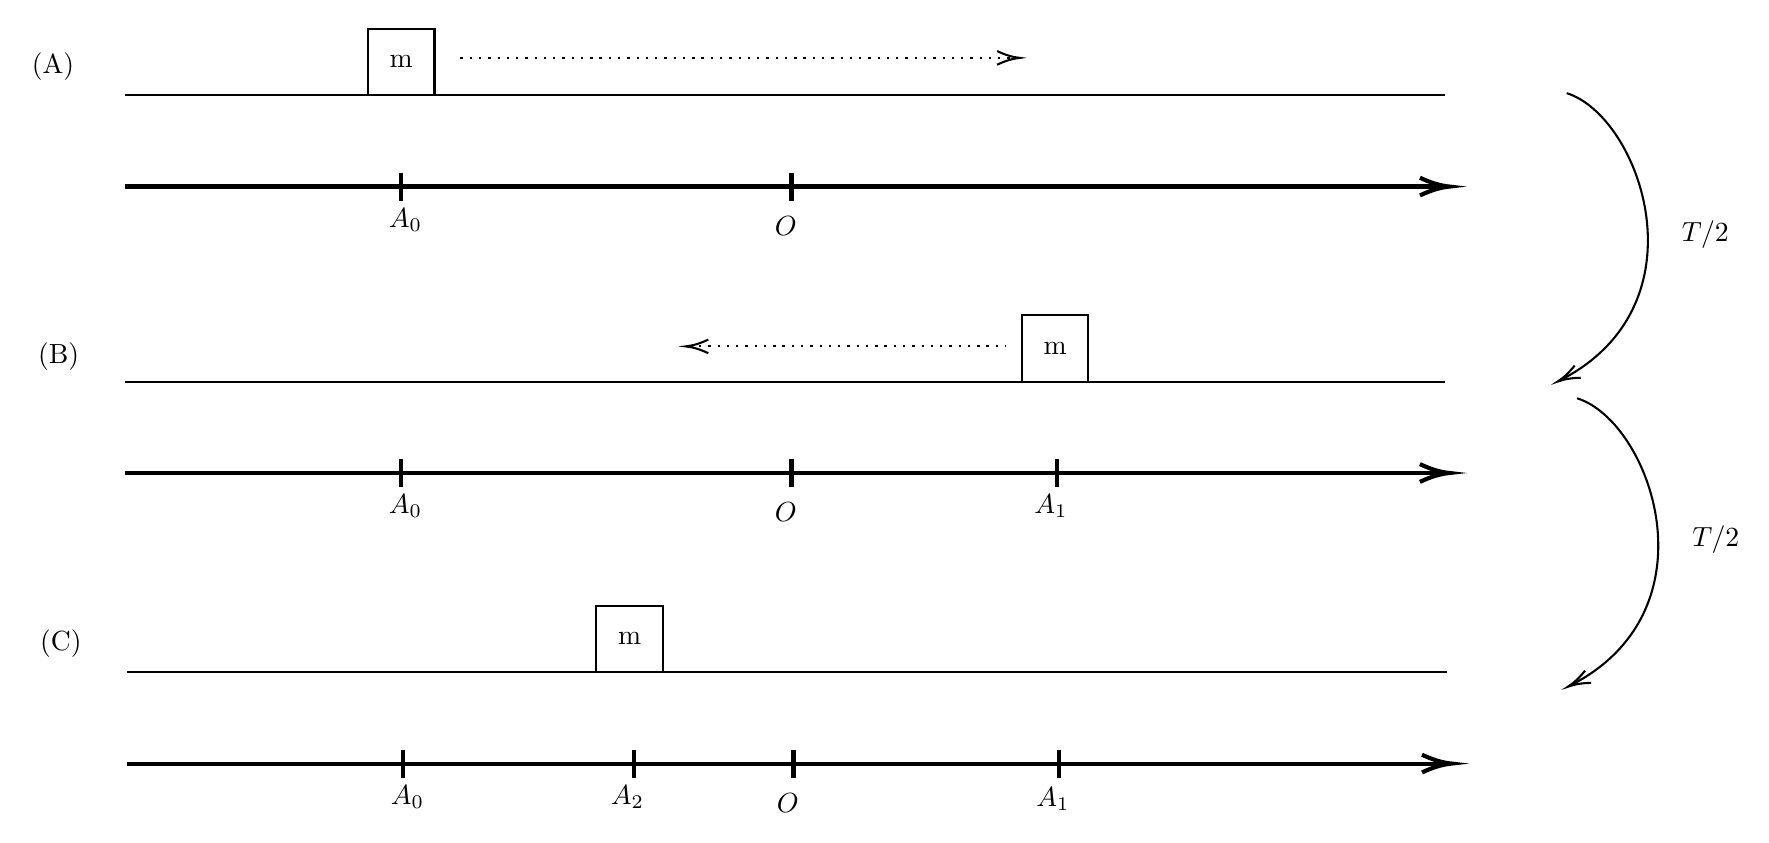
\begin{tikzpicture}[x=0.75pt,y=0.75pt,yscale=-1,xscale=1]
%uncomment if require: \path (0,15225); %set diagram left start at 0, and has height of 15225

%Straight Lines [id:da8440235981456923] 
\draw [color={rgb, 255:red, 0; green, 0; blue, 0 }  ,draw opacity=1 ]   (748.5,4556) -- (112.5,4556) ;
%Shape: Square [id:dp7730743948956422] 
\draw  [color={rgb, 255:red, 0; green, 0; blue, 0 }  ,draw opacity=1 ] (229.5,4524) -- (261.5,4524) -- (261.5,4556) -- (229.5,4556) -- cycle ;
%Straight Lines [id:da5849410238032737] 
\draw [color={rgb, 255:red, 0; green, 0; blue, 0 }  ,draw opacity=1 ][line width=1.5]    (433.5,4600) -- (747.5,4600) ;
\draw [shift={(750.5,4600)}, rotate = 180] [color={rgb, 255:red, 0; green, 0; blue, 0 }  ,draw opacity=1 ][line width=1.5]    (14.21,-4.28) .. controls (9.04,-1.82) and (4.3,-0.39) .. (0,0) .. controls (4.3,0.39) and (9.04,1.82) .. (14.21,4.28)   ;
%Straight Lines [id:da501337374602] 
\draw [color={rgb, 255:red, 0; green, 0; blue, 0 }  ,draw opacity=1 ][line width=1.5]    (245.5,4600) -- (433.5,4600) ;
\draw [shift={(433.5,4600)}, rotate = 180] [color={rgb, 255:red, 0; green, 0; blue, 0 }  ,draw opacity=1 ][line width=1.5]    (0,6.71) -- (0,-6.71)   ;
%Straight Lines [id:da8338549647082345] 
\draw [color={rgb, 255:red, 0; green, 0; blue, 0 }  ,draw opacity=1 ][line width=1.5]    (112.5,4600) -- (245.5,4600) ;
\draw [shift={(245.5,4600)}, rotate = 180] [color={rgb, 255:red, 0; green, 0; blue, 0 }  ,draw opacity=1 ][line width=1.5]    (0,6.71) -- (0,-6.71)   ;
%Straight Lines [id:da5472639759035778] 
\draw [color={rgb, 255:red, 0; green, 0; blue, 0 }  ,draw opacity=1 ]   (748.5,4694) -- (112.5,4694) ;
%Shape: Square [id:dp11345606497116645] 
\draw  [color={rgb, 255:red, 0; green, 0; blue, 0 }  ,draw opacity=1 ] (544.5,4662) -- (576.5,4662) -- (576.5,4694) -- (544.5,4694) -- cycle ;
%Straight Lines [id:da28185616117474566] 
\draw [color={rgb, 255:red, 0; green, 0; blue, 0 }  ,draw opacity=1 ][line width=1.5]    (433.5,4738) -- (747.5,4738) ;
\draw [shift={(750.5,4738)}, rotate = 180] [color={rgb, 255:red, 0; green, 0; blue, 0 }  ,draw opacity=1 ][line width=1.5]    (14.21,-4.28) .. controls (9.04,-1.82) and (4.3,-0.39) .. (0,0) .. controls (4.3,0.39) and (9.04,1.82) .. (14.21,4.28)   ;
%Straight Lines [id:da614812825007393] 
\draw [color={rgb, 255:red, 0; green, 0; blue, 0 }  ,draw opacity=1 ][line width=1.5]    (245.5,4738) -- (433.5,4738) ;
\draw [shift={(433.5,4738)}, rotate = 180] [color={rgb, 255:red, 0; green, 0; blue, 0 }  ,draw opacity=1 ][line width=1.5]    (0,6.71) -- (0,-6.71)   ;
%Straight Lines [id:da3151466941990222] 
\draw [color={rgb, 255:red, 0; green, 0; blue, 0 }  ,draw opacity=1 ][line width=1.5]    (112.5,4738) -- (245.5,4738) ;
\draw [shift={(245.5,4738)}, rotate = 180] [color={rgb, 255:red, 0; green, 0; blue, 0 }  ,draw opacity=1 ][line width=1.5]    (0,6.71) -- (0,-6.71)   ;
%Straight Lines [id:da16801387670839896] 
\draw [color={rgb, 255:red, 0; green, 0; blue, 0 }  ,draw opacity=1 ][line width=1.5]    (433.5,4738) -- (561.5,4738) ;
\draw [shift={(561.5,4738)}, rotate = 180] [color={rgb, 255:red, 0; green, 0; blue, 0 }  ,draw opacity=1 ][line width=1.5]    (0,6.71) -- (0,-6.71)   ;
%Straight Lines [id:da7824565205771314] 
\draw [color={rgb, 255:red, 0; green, 0; blue, 0 }  ,draw opacity=1 ]   (749.5,4834) -- (113.5,4834) ;
%Shape: Square [id:dp10726696816762793] 
\draw  [color={rgb, 255:red, 0; green, 0; blue, 0 }  ,draw opacity=1 ] (339.5,4802) -- (371.5,4802) -- (371.5,4834) -- (339.5,4834) -- cycle ;
%Straight Lines [id:da5556513504225804] 
\draw [color={rgb, 255:red, 0; green, 0; blue, 0 }  ,draw opacity=1 ][line width=1.5]    (434.5,4878) -- (748.5,4878) ;
\draw [shift={(751.5,4878)}, rotate = 180] [color={rgb, 255:red, 0; green, 0; blue, 0 }  ,draw opacity=1 ][line width=1.5]    (14.21,-4.28) .. controls (9.04,-1.82) and (4.3,-0.39) .. (0,0) .. controls (4.3,0.39) and (9.04,1.82) .. (14.21,4.28)   ;
%Straight Lines [id:da35868213260288484] 
\draw [color={rgb, 255:red, 0; green, 0; blue, 0 }  ,draw opacity=1 ][line width=1.5]    (246.5,4878) -- (434.5,4878) ;
\draw [shift={(434.5,4878)}, rotate = 180] [color={rgb, 255:red, 0; green, 0; blue, 0 }  ,draw opacity=1 ][line width=1.5]    (0,6.71) -- (0,-6.71)   ;
%Straight Lines [id:da9226047069569581] 
\draw [color={rgb, 255:red, 0; green, 0; blue, 0 }  ,draw opacity=1 ][line width=1.5]    (113.5,4878) -- (246.5,4878) ;
\draw [shift={(246.5,4878)}, rotate = 180] [color={rgb, 255:red, 0; green, 0; blue, 0 }  ,draw opacity=1 ][line width=1.5]    (0,6.71) -- (0,-6.71)   ;
%Straight Lines [id:da39824710137073915] 
\draw [color={rgb, 255:red, 0; green, 0; blue, 0 }  ,draw opacity=1 ][line width=1.5]    (434.5,4878) -- (562.5,4878) ;
\draw [shift={(562.5,4878)}, rotate = 180] [color={rgb, 255:red, 0; green, 0; blue, 0 }  ,draw opacity=1 ][line width=1.5]    (0,6.71) -- (0,-6.71)   ;
%Straight Lines [id:da5711245809745336] 
\draw [color={rgb, 255:red, 0; green, 0; blue, 0 }  ,draw opacity=1 ][line width=1.5]    (357.5,4878) -- (434.5,4878) ;
\draw [shift={(357.5,4878)}, rotate = 180] [color={rgb, 255:red, 0; green, 0; blue, 0 }  ,draw opacity=1 ][line width=1.5]    (0,6.71) -- (0,-6.71)   ;
%Straight Lines [id:da2785554999977735] 
\draw [color={rgb, 255:red, 0; green, 0; blue, 0 }  ,draw opacity=1 ] [dash pattern={on 0.84pt off 2.51pt}]  (274,4538) -- (541.5,4538) ;
\draw [shift={(543.5,4538)}, rotate = 180] [color={rgb, 255:red, 0; green, 0; blue, 0 }  ,draw opacity=1 ][line width=0.75]    (10.93,-3.29) .. controls (6.95,-1.4) and (3.31,-0.3) .. (0,0) .. controls (3.31,0.3) and (6.95,1.4) .. (10.93,3.29)   ;
%Straight Lines [id:da5363770674501016] 
\draw [color={rgb, 255:red, 0; green, 0; blue, 0 }  ,draw opacity=1 ] [dash pattern={on 0.84pt off 2.51pt}]  (384.5,4677) -- (536.5,4677) ;
\draw [shift={(382.5,4677)}, rotate = 0] [color={rgb, 255:red, 0; green, 0; blue, 0 }  ,draw opacity=1 ][line width=0.75]    (10.93,-3.29) .. controls (6.95,-1.4) and (3.31,-0.3) .. (0,0) .. controls (3.31,0.3) and (6.95,1.4) .. (10.93,3.29)   ;
%Curve Lines [id:da8774718138615303] 
\draw [color={rgb, 255:red, 0; green, 0; blue, 0 }  ,draw opacity=1 ]   (807,4555) .. controls (842.32,4565.95) and (875.17,4657.08) .. (803.59,4693.46) ;
\draw [shift={(802.5,4694)}, rotate = 333.75] [color={rgb, 255:red, 0; green, 0; blue, 0 }  ,draw opacity=1 ][line width=0.75]    (10.93,-3.29) .. controls (6.95,-1.4) and (3.31,-0.3) .. (0,0) .. controls (3.31,0.3) and (6.95,1.4) .. (10.93,3.29)   ;
%Curve Lines [id:da6809827298064757] 
\draw [color={rgb, 255:red, 0; green, 0; blue, 0 }  ,draw opacity=1 ]   (812,4702) .. controls (847.32,4712.95) and (880.17,4804.08) .. (808.59,4840.46) ;
\draw [shift={(807.5,4841)}, rotate = 333.75] [color={rgb, 255:red, 0; green, 0; blue, 0 }  ,draw opacity=1 ][line width=0.75]    (10.93,-3.29) .. controls (6.95,-1.4) and (3.31,-0.3) .. (0,0) .. controls (3.31,0.3) and (6.95,1.4) .. (10.93,3.29)   ;

% Text Node
\draw (245.5,4540) node   [align=left] {\textcolor{black}{m}};
% Text Node
\draw (424,4613) node [anchor=north west][inner sep=0.75pt]    {\textcolor{black}{$O$}};
% Text Node
\draw (238,4609) node [anchor=north west][inner sep=0.75pt]    {\textcolor{black}{$A_{0}$}};
% Text Node
\draw (560.5,4678) node   [align=left] {\textcolor{black}{m}};
% Text Node
\draw (424,4751) node [anchor=north west][inner sep=0.75pt]    {\textcolor{black}{$O$}};
% Text Node
\draw (238,4747) node [anchor=north west][inner sep=0.75pt]    {\textcolor{black}{$A_{0}$}};
% Text Node
\draw (549,4747) node [anchor=north west][inner sep=0.75pt]    {\textcolor{black}{$A_{1}$}};
% Text Node
\draw (355.5,4818) node   [align=left] {\textcolor{black}{m}};
% Text Node
\draw (425,4891) node [anchor=north west][inner sep=0.75pt]    {\textcolor{black}{$O$}};
% Text Node
\draw (239,4887) node [anchor=north west][inner sep=0.75pt]    {\textcolor{black}{$A_{0}$}};
% Text Node
\draw (550,4888) node [anchor=north west][inner sep=0.75pt]    {\textcolor{black}{$A_{1}$}};
% Text Node
\draw (345,4887) node [anchor=north west][inner sep=0.75pt]    {\textcolor{black}{$A_{2}$}};
% Text Node
\draw (861,4615) node [anchor=north west][inner sep=0.75pt]    {\textcolor{black}{$T/2$}};
% Text Node
\draw (866,4762) node [anchor=north west][inner sep=0.75pt]    {\textcolor{black}{$T/2$}};
% Text Node
\draw (66,4534) node [anchor=north west][inner sep=0.75pt]   [align=left] {(A)};
% Text Node
\draw (69,4674) node [anchor=north west][inner sep=0.75pt]   [align=left] {(B)};
% Text Node
\draw (70,4812) node [anchor=north west][inner sep=0.75pt]   [align=left] {(C)};


\end{tikzpicture}}
    \caption{}
    \label{fig:1.5}
\end{figure}

Vậy thì ta có công thức liên hệ giữa các biên độ liền kề nhau.

\begin{equation}
    A_{k+1} = A_{k} - 2 \mu mg/k.
\end{equation}


\subsubsection{Lực ma sát nhớt}
\label{sec:1.2.2}

\begin{figure}[!htb]
    \centering
    \definecolor{wsdred}{HTML}{8E1728}



% Pattern Info
 
\tikzset{
pattern size/.store in=\mcSize, 
pattern size = 5pt,
pattern thickness/.store in=\mcThickness, 
pattern thickness = 0.3pt,
pattern radius/.store in=\mcRadius, 
pattern radius = 1pt}
\makeatletter
\pgfutil@ifundefined{pgf@pattern@name@_hkp691r1q}{
\pgfdeclarepatternformonly[\mcThickness,\mcSize]{_hkp691r1q}
{\pgfqpoint{0pt}{0pt}}
{\pgfpoint{\mcSize+\mcThickness}{\mcSize+\mcThickness}}
{\pgfpoint{\mcSize}{\mcSize}}
{
\pgfsetcolor{\tikz@pattern@color}
\pgfsetlinewidth{\mcThickness}
\pgfpathmoveto{\pgfqpoint{0pt}{0pt}}
\pgfpathlineto{\pgfpoint{\mcSize+\mcThickness}{\mcSize+\mcThickness}}
\pgfusepath{stroke}
}}
\makeatother
\tikzset{every picture/.style={line width=0.75pt}} %set default line width to 0.75pt        

\begin{tikzpicture}[x=0.75pt,y=0.75pt,yscale=-1,xscale=1]
%uncomment if require: \path (0,15225); %set diagram left start at 0, and has height of 15225

%Straight Lines [id:da37304025889826953] 
\draw [color={rgb, 255:red, 0; green, 0; blue, 0 }  ,draw opacity=1 ]   (655.5,345.22) -- (656,430.22) ;
%Straight Lines [id:da5291924352353508] 
\draw [color={rgb, 255:red, 0; green, 0; blue, 0 }  ,draw opacity=1 ]   (881.5,430.22) -- (656,430.22) ;
%Shape: Rectangle [id:dp36057955226019] 
\draw  [draw opacity=0][pattern=_hkp691r1q,pattern size=6pt,pattern thickness=0.75pt,pattern radius=0pt, pattern color={rgb, 255:red, 0; green, 0; blue, 0}] (655.5,345.22) -- (630.5,345.22) -- (630.5,430.22) -- (655.5,430.22) -- cycle ;
%Shape: Resistor [id:dp17501377685772912] 
\draw  [color={rgb, 255:red, 0; green, 0; blue, 0 }  ,draw opacity=1 ] (655.75,371.72) -- (672.4,371.72) -- (676.1,362.84) -- (683.5,380.59) -- (690.9,362.84) -- (698.3,380.59) -- (705.7,362.84) -- (713.1,380.59) -- (720.5,362.84) -- (727.9,380.59) -- (731.6,371.72) -- (748.25,371.72) ;
%Shape: Square [id:dp0196154664863446] 
\draw  [color={rgb, 255:red, 0; green, 0; blue, 0 }  ,draw opacity=1 ] (748.5,345.22) -- (833.5,345.22) -- (833.5,430.22) -- (748.5,430.22) -- cycle ;
%Straight Lines [id:da8181933130785954] 
\draw [color={rgb, 255:red, 0; green, 0; blue, 0 }  ,draw opacity=1 ]   (900.5,460.22) -- (794.5,460.22) ;
\draw [shift={(794.5,460.22)}, rotate = 360] [color={rgb, 255:red, 0; green, 0; blue, 0 }  ,draw opacity=1 ][line width=0.75]    (0,5.59) -- (0,-5.59)   ;
\draw [shift={(903.5,460.22)}, rotate = 180] [fill={rgb, 255:red, 0; green, 0; blue, 0 }  ,fill opacity=1 ][line width=0.08]  [draw opacity=0] (8.93,-4.29) -- (0,0) -- (8.93,4.29) -- cycle    ;
%Straight Lines [id:da9897224429030973] 
\draw [color={rgb, 255:red, 0; green, 0; blue, 0 }  ,draw opacity=1 ]   (794.5,460.22) -- (685.5,460.22) ;
%Straight Lines [id:da820285675152675] 
\draw [color={rgb, 255:red, 0; green, 0; blue, 0 }  ,draw opacity=1 ]   (656.5,418.22) -- (692.5,418.22) ;
%Straight Lines [id:da2106300828191292] 
\draw [color={rgb, 255:red, 0; green, 0; blue, 0 }  ,draw opacity=1 ]   (709.5,418.22) -- (747.5,418.22) ;
%Shape: Rectangle [id:dp8209831967221957] 
\draw  [color={rgb, 255:red, 0; green, 0; blue, 0 }  ,draw opacity=1 ][fill={rgb, 255:red, 155; green, 155; blue, 155 }  ,fill opacity=1 ][line width=0.75]  (707.42,414.02) -- (713.5,414.02) -- (713.5,423.22) -- (707.42,423.22) -- cycle ;
%Straight Lines [id:da48698349083621584] 
\draw [color={rgb, 255:red, 0; green, 0; blue, 0 }  ,draw opacity=1 ][line width=0.75]    (692,410.62) -- (717.96,410.62) ;
%Straight Lines [id:da6988678110798234] 
\draw [color={rgb, 255:red, 0; green, 0; blue, 0 }  ,draw opacity=1 ][line width=0.75]    (692.51,410.22) -- (692.51,426.22) ;
%Straight Lines [id:da7874952591280222] 
\draw [color={rgb, 255:red, 0; green, 0; blue, 0 }  ,draw opacity=1 ][line width=0.75]    (692.51,425.82) -- (718.47,425.82) ;

%Straight Lines [id:da48875406084702644] 
\draw [color={rgb, 255:red, 65; green, 117; blue, 5 }  ,draw opacity=1 ][line width=2.25]    (748.5,418.22) -- (729.5,418.05) ;
\draw [shift={(724.5,418)}, rotate = 0.52] [fill={rgb, 255:red, 65; green, 117; blue, 5 }  ,fill opacity=1 ][line width=0.08]  [draw opacity=0] (14.29,-6.86) -- (0,0) -- (14.29,6.86) -- cycle    ;
%Straight Lines [id:da5308011266026909] 
\draw [color={wsdred}  ,draw opacity=1 ][line width=1.5]    (833,388) -- (854.5,388) ;
\draw [shift={(858.5,388)}, rotate = 180] [fill={wsdred}  ,fill opacity=1 ][line width=0.08]  [draw opacity=0] (11.61,-5.58) -- (0,0) -- (11.61,5.58) -- cycle    ;

% Text Node
\draw (697,335.22) node [anchor=north west][inner sep=0.75pt]   [align=left] {k};
% Text Node
\draw (791,387.72) node   [align=left] {m};
% Text Node
\draw (794.5,465.22) node [anchor=north] [inner sep=0.75pt]   [align=left] {O};
% Text Node
\draw (696,387.22) node [anchor=north west][inner sep=0.75pt]   [align=left] {b};
% Text Node
\draw (726,386) node [anchor=north west][inner sep=0.75pt]  [color={rgb, 255:red, 102; green, 170; blue, 27 }  ,opacity=1 ]  {$F_{2}$};
% Text Node
\draw (839,359) node [anchor=north west][inner sep=0.75pt]  {$\vec{v}$};


\end{tikzpicture}
    \caption{}
\end{figure}

Lực ma sát nhớt sẽ bị phụ vào độ lớn và hướng của vận tốc hệ vật theo biểu thức sau. Ở đây lực ma sát nhớt mà chúng ta khảo sát là lực phụ thuộc bậc 1 vào vận tốc hệ vật\footnote{Tồn tại lực ma sát nhớt phụ thuộc bậc 2 vào vận tốc vật. Nhưng trong bài toán này ta không xét tới.}. 
\begin{equation}
    \vec{F}_2 = - b \vec{v}.
    \label{eq:1.8}
\end{equation}
Ta có thể viết được phương trình vi phân chuyển động của nó.
\begin{equation*}
    m \ddot{x} = - k x - b \dot{x}.
\end{equation*}
Đây chính là phương trình vi phân bậc 2, để trở thành đúng dạng đã học thì ta sẽ ghi thành
\begin{equation}
    \ddot{x} + {\displaystyle \frac{b}{m}} \dot{x} + {\displaystyle \frac{k}{m}} x = 0. 
    \label{eq:1.9}
\end{equation}
Ta giả sử \(x = A e^{\lambda t}\). Thay nó vào phương trình \ref{eq:1.9}. Ta đặt \(b/m = 2 \gamma\), \(\omega = \sqrt{k/m}\).
\begin{equation*}
    \lambda^2 + (2\gamma) \lambda + \omega^2 = 0.
\end{equation*}

Tính \(\Delta\) của phương trình bậc 2, ta thu được
\begin{equation}
    \Delta = 4 \gamma^2 - 4 \omega^2
    \label{eq:1.10}
\end{equation}
\vspace{2mm}

\underline{\textit{Trường hợp (1): $\Delta$ < 0 - Lực cản nhỏ}}

Ta thu được \(\lambda\) và nghiệm tổng quát của phương trình vi phân.
\begin{equation}
    \left\{
    \begin{array}{ccc}
    \lambda &=& - \gamma \pm  i \sqrt{\omega^2 - \gamma^2} \\
    x &=& e^{-\gamma t} \left(A e^{i\sqrt{\omega^2 - \gamma^2} \ t} + B e^{- i\sqrt{\omega^2 - \gamma^2} \ t} \right).
    \end{array}
    \right.
    \label{eq:1.11}
\end{equation}

Nhưng kết quả ta thu được buộc phải là số thực, vậy nên các hằng số $A, B$ sẽ đảm bảo cho $x$ là một số thực. Cụ thể thì $A$ và $B$ phải có liên hệ
\begin{equation*}
    \left\{
    \begin{array}{ccc}
    A + B &=& C \cos \phi \\
    A - B &=& i C \sin \phi
    \end{array}
    \right.
\end{equation*}
Vậy thì ta sẽ thu được nghiệm tổng quát \(x\) như sau
\begin{equation}
\begin{split}
    x = e^{-\gamma t} C \cos{\left(\sqrt{\omega^2 - \gamma^2} \ t + \phi \right)}
\end{split}
\label{eq:1.12}
\end{equation}

\begin{figure}[!htb]
    \centering
    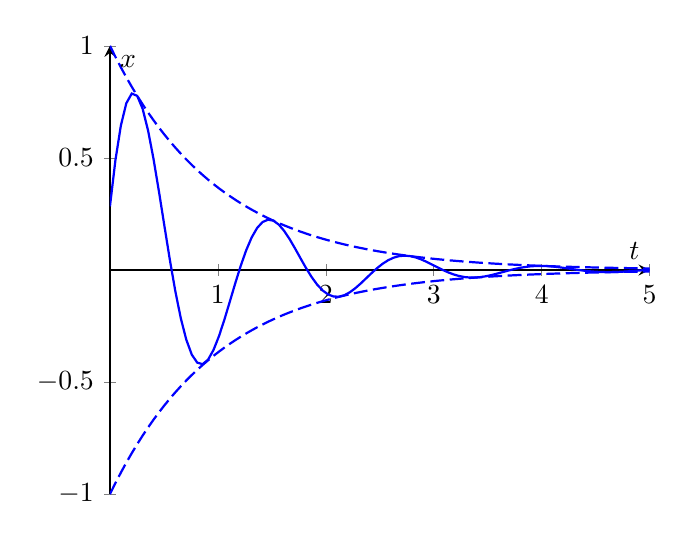
\begin{tikzpicture}[scale=1]
      \begin{axis}[
          domain=0:5,
          samples=100,
          axis lines=middle,
          xlabel=$t$,
          ylabel=$x$
        ]
        \addplot[blue, thick, dash pattern=on 5pt off 2pt] {e^(-x)};
        \addplot[blue, thick, dash pattern=on 5pt off 2pt] {-e^(-x)};
        \addplot[blue, thick] {e^(-x)*cos(deg(5*x + 5))};
      \end{axis}
    \end{tikzpicture}
    \caption{Hàm \(e^{-t} \cos{\left(5t + 5 \right)}\)}
    \label{fig:1.6}
\end{figure}

\newpage
\vspace{2mm}

\underline{\textit{Trường hợp (2): \(\Delta\) > 0 - Lực cản lớn}}

Ta thu được \(\lambda\) và nghiệm tổng quát của phương trình vi phân.
\begin{equation}
    \left\{
    \begin{array}{ccc}
    \lambda &=& - \gamma \pm   \sqrt{\gamma^2 - \omega^2} \\
    x &=& A e^{- \left( \gamma - \sqrt{\gamma^2 - \omega^2}\right)  t} + B e^{- \left( \gamma + \sqrt{\gamma^2 - \omega^2}\right) t}.
    \end{array}
    \right.
    \label{eq:1.13}
\end{equation}

Trong trường hợp lực cản lớn, vật sẽ không thực hiện quá trình dao động. Mà bị tắt dần (nhưng chậm).

\begin{figure}[!htb]
    \centering
    \begin{tikzpicture}[scale=1]
      \begin{axis}[
          domain=0:2,
          samples=100,
          axis lines=middle,
          xlabel=$t$,
          ylabel=$x$
        ]
        \addplot[blue, thick] {20*e^(-(5-2)*x) +10*e^(-(5+2)*x};
      \end{axis}
    \end{tikzpicture}
    \caption{Hàm \(20 e^{-(5-2)t} + 10 e^{-(5+2)t}\)}
    \label{fig:1.7}
\end{figure}
\vspace{2mm}

\underline{\textit{Trường hợp (3): \(\Delta = 0\) - Tới hạn}}

Trong trường hợp này, khi ta giải phương trình bậc 2 nó sẽ bị trùng nghiệm. Và ta sẽ không thể áp dụng cách đã làm với trường hợp (1) và (2) vào đây được. Lúc này, dựa vào lý thuyết để giải phương trình vi phân, ta sẽ biết dạng tổng quát của \(x\). Chuyển động sẽ tắt dần rất nhanh. 
\begin{equation}
    \left\{
    \begin{array}{ccc}
    \lambda &=& \omega = \gamma \\
    x &=& e^{-\gamma t} \left( A + B t\right).
    \end{array}
    \right.
    \label{eq:1.14}
\end{equation}

\begin{figure}[!htb]
    \centering
    \begin{tikzpicture}[scale=1]
      \begin{axis}[
          domain=0:2,
          samples=100,
          axis lines=middle,
          xlabel=$t$,
          ylabel=$x$
        ]
        \addplot[blue, thick] {e^(-5*x)*(20 + 10*x)};
      \end{axis}
    \end{tikzpicture}
    \caption{Hàm \(e^{-5t} \left(20 + 10t\right)\)}
    \label{fig:1.8}
\end{figure}
\vspace{2mm}

Tóm lại, với trường hợp có lực cản nhớt trong hệ thì ta có một vài trường hợp xảy ra. Từ đấy, ta tổng hợp thành một bảng. Xét phương trình đặc trưng của phương trình vi phân bậc 2 là:
\begin{equation*}
    a\lambda^2 + b\lambda + c = 0 
\end{equation*}

\begin{table}[!htb]
    \centering
    \caption{Tóm tắt nghiệm}
    \definecolor{wsdred}{HTML}{8E1728}



\tikzset{every picture/.style={line width=0.75pt}} %set default line width to 0.75pt        

\begin{tikzpicture}[x=0.75pt,y=0.75pt,yscale=-1,xscale=1]
%uncomment if require: \path (0,15225); %set diagram left start at 0, and has height of 15225

%Shape: Rectangle [id:dp023490157006617496] 
\draw   (86,3178) -- (425.25,3178) -- (425.25,3204.61) -- (86,3204.61) -- cycle ;
%Shape: Rectangle [id:dp22955898152245124] 
\draw   (425.25,3178) -- (764.5,3178) -- (764.5,3204.61) -- (425.25,3204.61) -- cycle ;
%Shape: Rectangle [id:dp15936845341682115] 
\draw   (86,3204.61) -- (425.25,3204.61) -- (425.25,3268.07) -- (86,3268.07) -- cycle ;
%Shape: Rectangle [id:dp25816905700698767] 
\draw   (425.25,3204.61) -- (764.5,3204.61) -- (764.5,3268.07) -- (425.25,3268.07) -- cycle ;
%Shape: Rectangle [id:dp3735020094318289] 
\draw   (86,3268.07) -- (425.25,3268.07) -- (425.25,3350.51) -- (86,3350.51) -- cycle ;
%Shape: Rectangle [id:dp031979667412538104] 
\draw   (425.25,3268.07) -- (764.5,3268.07) -- (764.5,3350.51) -- (425.25,3350.51) -- cycle ;
%Shape: Rectangle [id:dp0818394520455934] 
\draw   (86,3350.51) -- (425.25,3350.51) -- (425.25,3439) -- (86,3439) -- cycle ;
%Shape: Rectangle [id:dp13005863494043002] 
\draw   (425.25,3350.51) -- (764.5,3350.51) -- (764.5,3439) -- (425.25,3439) -- cycle ;

% Text Node
\draw (201,3180) node [anchor=north west][inner sep=0.75pt]   [align=left] {Trường hợp};
% Text Node
\draw (205,3225) node [anchor=north west][inner sep=0.75pt]   [align=left] {Vô nghiệm};
% Text Node
\draw (543,3180) node [anchor=north west][inner sep=0.75pt]   [align=left] {Nghiệm tổng quát};
% Text Node
\draw (439,3213.05) node [anchor=north west][inner sep=0.75pt]    {$x\ =C\ \exp\left(\displaystyle -\frac{b}{2a} \ t\right) \ \cos\left(\sqrt{4ac\ -\ b^{2}} \ t\ +\phi \right)$};
% Text Node
\draw (178,3273) node [anchor=north west][inner sep=0.75pt]   [align=left] {2 nghiệm phân biệt};
% Text Node
\draw (439,3297.05) node [anchor=north west][inner sep=0.75pt]    {$x\ =A e^{\lambda _{1}  t} \ +\ B e^{\lambda _{2}  t}$};
% Text Node
\draw (179,3294.67) node [anchor=north west][inner sep=0.75pt]   [align=left] {$\displaystyle \lambda \ =\ \frac{-\ b\ \pm \ \sqrt{\Delta }}{2a}$};
% Text Node
\draw (174,3359) node [anchor=north west][inner sep=0.75pt]   [align=left] {1 nghiệm duy nhất};
% Text Node
\draw (179,3385.84) node [anchor=north west][inner sep=0.75pt]   [align=left] {$\displaystyle \lambda \ =\ -\ \frac{b}{2a}$};
% Text Node
\draw (436,3381.05) node [anchor=north west][inner sep=0.75pt]    {$x\ =\ e^{-\lambda  t}  (  A+ B t) \ $};


\end{tikzpicture}
    \label{tab:1.7}
\end{table}

**Trong đó, \(A, B, C, \phi\) là những hằng số dựa vào những điều kiện biên đề cho.

\subsection{Dao động có lực cưỡng bức}
Khi này, hệ vật chịu thêm một lực từ một nguồn khác. Lực này có dạng là một dạng lực điều hoà.
\begin{equation}
    F(t) = F_0 \cos{\left(\Omega t + \phi \right)}.
    \label{eq:1.15}
\end{equation}

\begin{figure}[!htb]
    \centering
    \definecolor{wsdred}{HTML}{8E1728}



% Pattern Info
 
\tikzset{
pattern size/.store in=\mcSize, 
pattern size = 5pt,
pattern thickness/.store in=\mcThickness, 
pattern thickness = 0.3pt,
pattern radius/.store in=\mcRadius, 
pattern radius = 1pt}
\makeatletter
\pgfutil@ifundefined{pgf@pattern@name@_o3npe040r}{
\pgfdeclarepatternformonly[\mcThickness,\mcSize]{_o3npe040r}
{\pgfqpoint{0pt}{0pt}}
{\pgfpoint{\mcSize+\mcThickness}{\mcSize+\mcThickness}}
{\pgfpoint{\mcSize}{\mcSize}}
{
\pgfsetcolor{\tikz@pattern@color}
\pgfsetlinewidth{\mcThickness}
\pgfpathmoveto{\pgfqpoint{0pt}{0pt}}
\pgfpathlineto{\pgfpoint{\mcSize+\mcThickness}{\mcSize+\mcThickness}}
\pgfusepath{stroke}
}}
\makeatother
\tikzset{every picture/.style={line width=0.75pt}} %set default line width to 0.75pt        

\begin{tikzpicture}[x=0.75pt,y=0.75pt,yscale=-1,xscale=1]
%uncomment if require: \path (0,15225); %set diagram left start at 0, and has height of 15225

%Straight Lines [id:da03890405315517542] 
\draw [color={rgb, 255:red, 0; green, 0; blue, 0 }  ,draw opacity=1 ]   (77.5,595.22) -- (78,680.22) ;
%Straight Lines [id:da6771080202521618] 
\draw [color={rgb, 255:red, 0; green, 0; blue, 0 }  ,draw opacity=1 ]   (303.5,680.22) -- (78,680.22) ;
%Shape: Rectangle [id:dp8957593748114105] 
\draw  [draw opacity=0][pattern=_o3npe040r,pattern size=6pt,pattern thickness=0.75pt,pattern radius=0pt, pattern color={rgb, 255:red, 0; green, 0; blue, 0}] (77.5,595.22) -- (52.5,595.22) -- (52.5,680.22) -- (77.5,680.22) -- cycle ;
%Shape: Resistor [id:dp9587285208573366] 
\draw  [color={rgb, 255:red, 0; green, 0; blue, 0 }  ,draw opacity=1 ] (77.75,621.72) -- (94.4,621.72) -- (98.1,612.84) -- (105.5,630.59) -- (112.9,612.84) -- (120.3,630.59) -- (127.7,612.84) -- (135.1,630.59) -- (142.5,612.84) -- (149.9,630.59) -- (153.6,621.72) -- (170.25,621.72) ;
%Shape: Square [id:dp46764462046986255] 
\draw  [color={rgb, 255:red, 0; green, 0; blue, 0 }  ,draw opacity=1 ] (170.5,595.22) -- (255.5,595.22) -- (255.5,680.22) -- (170.5,680.22) -- cycle ;
%Straight Lines [id:da1727736810609144] 
\draw [color={rgb, 255:red, 0; green, 0; blue, 0 }  ,draw opacity=1 ]   (322.5,710.22) -- (216.5,710.22) ;
\draw [shift={(216.5,710.22)}, rotate = 360] [color={rgb, 255:red, 0; green, 0; blue, 0 }  ,draw opacity=1 ][line width=0.75]    (0,5.59) -- (0,-5.59)   ;
\draw [shift={(325.5,710.22)}, rotate = 180] [fill={rgb, 255:red, 0; green, 0; blue, 0 }  ,fill opacity=1 ][line width=0.08]  [draw opacity=0] (8.93,-4.29) -- (0,0) -- (8.93,4.29) -- cycle    ;
%Straight Lines [id:da5324610265708711] 
\draw [color={rgb, 255:red, 0; green, 0; blue, 0 }  ,draw opacity=1 ]   (216.5,710.22) -- (107.5,710.22) ;
%Straight Lines [id:da24682222137677545] 
\draw [color={rgb, 255:red, 0; green, 0; blue, 0 }  ,draw opacity=1 ]   (78.5,668.22) -- (114.5,668.22) ;
%Straight Lines [id:da08809092762479498] 
\draw [color={rgb, 255:red, 0; green, 0; blue, 0 }  ,draw opacity=1 ]   (131.5,668.22) -- (169.5,668.22) ;
%Shape: Rectangle [id:dp729685852038932] 
\draw  [color={rgb, 255:red, 0; green, 0; blue, 0 }  ,draw opacity=1 ][fill={rgb, 255:red, 155; green, 155; blue, 155 }  ,fill opacity=1 ][line width=0.75]  (129.42,664.02) -- (135.5,664.02) -- (135.5,673.22) -- (129.42,673.22) -- cycle ;
%Straight Lines [id:da9203533268837498] 
\draw [color={rgb, 255:red, 0; green, 0; blue, 0 }  ,draw opacity=1 ][line width=0.75]    (114,660.62) -- (139.96,660.62) ;
%Straight Lines [id:da1854839912471089] 
\draw [color={rgb, 255:red, 0; green, 0; blue, 0 }  ,draw opacity=1 ][line width=0.75]    (114.51,660.22) -- (114.51,676.22) ;
%Straight Lines [id:da7739527238409212] 
\draw [color={rgb, 255:red, 0; green, 0; blue, 0 }  ,draw opacity=1 ][line width=0.75]    (114.51,675.82) -- (140.47,675.82) ;

%Straight Lines [id:da7046823744172879] 
\draw [line width=2.25]    (255,641) -- (294.5,641) ;
\draw [shift={(299.5,641)}, rotate = 180] [fill={wsdred}  ][line width=0.08]  [draw opacity=0] (14.29,-6.86) -- (0,0) -- (14.29,6.86) -- cycle    ;

% Text Node
\draw (119,585.22) node [anchor=north west][inner sep=0.75pt]   [align=left] {\textcolor{black}{k}};
% Text Node
\draw (213,637.72) node   [align=left] {M};
% Text Node
\draw (216.5,717) node [anchor=north] [inner sep=0.75pt]   [align=left] {\textcolor{black}{O}};
% Text Node
\draw (118,637.22) node [anchor=north west][inner sep=0.75pt]   [align=left] {\textcolor{black}{b}};
% Text Node
\draw (291,601) node [anchor=north west][inner sep=0.75pt]    {$\vec{F} \ =\ F_{0} \ \cos( \si{\ohm}t + \phi) \ \overrightarrow{e_{x}}$};


\end{tikzpicture}
    \caption{}
    \label{fig:1.9}
\end{figure}

Lực này cưỡng bức vật và khiến cho chuyển động theo có xu hướng theo chu kỳ của lực cưỡng bức. Ta viết phương trình vi phân chuyển động của hệ.
\begin{equation}
    m \ddot{x} + b \dot{x} + k x  = F_0 \cos{\left(\Omega t + \phi \right)}.
    \label{eq:1.16}
\end{equation}
Để giải quyết phương trình này, ta sẽ giải lần lượt nghiệm thuần nhất và nghiệm riêng của nó.
\vspace{2mm}

\underline{\textit{Nghiệm thuần nhất}}

Đặt nghiệm thuần nhất là \(x_{tn}\). Ta sẽ giải phương trình sau.
\begin{equation}
    \ddot{x}_{tn} + {\displaystyle \frac{b}{m}} \dot{x}_{tn} + {\displaystyle \frac{k}{m}} x_{tn} = 0.
    \label{eq:1.17}
\end{equation}
Phương trình này sẽ được giải quyết giống như mục (\ref{sec:1.2.2}). 
\vspace{2mm}

\underline{\textit{Nghiệm riêng}}

Đặt nghiệm riêng là \(x_r\). Nghiệm riêng sẽ mang đặc trưng của lực cưỡng bức. Hiểu đơn giản là nếu thế $x_r$ vào vế trái phương trình \ref{eq:1.16} nó sẽ thu gọn thành vế phải. Vì \(x_r\) mang đặc trưng của hàm lực cưỡng bức nên ta giả sử \(x_r\) có dạng sau.
\begin{equation}
    x_r = A \cos{\left(\Omega t + \phi\right)} + B \sin{\left(\Omega t + \phi \right)}.
    \label{eq:1.18}
\end{equation}

Thế phương trình \ref{eq:1.18} vào phương trình \ref{eq:1.16}. Rồi ta đồng nhất hai vế. Ở đây, đồng nhất hai vế là hệ số đi với cos() ở hai vế sẽ bằng nhau; hệ số đi với sin() ở hai vế sẽ bằng nhau.

\begin{equation*}
    \left(-A \Omega^2 + {\displaystyle \frac{b}{m}} B \Omega + {\displaystyle \frac{k}{m}} A  \right) \cos{\left(\Omega t + \phi \right)} + \left(-B \Omega^2 - {\displaystyle \frac{b}{m}} A \Omega + {\displaystyle \frac{k}{m}} B \right) \sin{\left(\Omega t + \phi\right)} = {\displaystyle \frac{F_0}{m}} \cos{\left(\Omega t + \phi \right)}.
\end{equation*}
Đồng nhất ta có
\begin{equation*}
\left\{
    \begin{array}{ccc}
    -A \Omega^2 + {\displaystyle \frac{b}{m}} B \Omega + {\displaystyle \frac{k}{m}} A  &=& {\displaystyle \frac{F_0}{m}} 
    \\
    \\
    -B \Omega^2 - {\displaystyle \frac{b}{m}} A \Omega + {\displaystyle \frac{k}{m}} B  &=& 0.
    \end{array}
\right.         
\end{equation*}
Để dễ biểu diễn, ta đặt \(c = b/m; \omega^2 = k/m\)
\begin{equation}
    \begin{array}{ccc}
    A &=& \displaystyle \frac{F_0}{m} \frac{\omega^2 - \Omega^2}{\left(\omega^2 - \Omega^2 \right)^2 + \left( c \Omega \right)^2}. 
    \\
    \\
    B &=& \displaystyle \frac{F_0}{m} \frac{c \Omega}{\left(\omega^2 - \Omega^2 \right)^2 + \left( c \Omega \right)^2}.
    \end{array}
    \label{eq:1.19}
\end{equation}
Vậy ta sẽ tìm được dạng của nghiệm riêng khi thế \(A, B\) vào phương trình \ref{eq:1.18}. 
\vspace{2mm}

\underline{\textit{Nghiệm tổng quát}}

Đặt nghiệm tổng quát là \(x\), ta sẽ tính được nghiệm tổng quát bằng biểu thức
\begin{equation}
    x = x_{tn} + x_r.
\end{equation}

Đây là lý thuyết trong việc giải các phương trình vi phân. Nghiệm tổng quát của phương trình vi phân tuyến tính sẽ là tổng các nghiệm. Một chú thích của mình để khiến cho các bạn đọc thấy được điều này một các trực quan hơn
\begin{equation*}
\begin{array}{cc}
    &m (\ddot{x}_{tn} + \ddot{x}_r) + b (\dot{x}_{tn} + \dot{x}_r) + k (x_{tn} + x_{r})  = F_0 \cos{\left(\Omega t + \phi \right)}. 
    \\
    \\
    
    \Leftrightarrow &  \left( \ddot{x}_{tn} + {\displaystyle \frac{b}{m}} \dot{x}_{tn} + {\displaystyle \frac{k}{m}} x_{tn}\right) + \left(    \ddot{x}_{r} + {\displaystyle \frac{b}{m}} \dot{x}_{r} + {\displaystyle \frac{k}{m}} x_{r} \right) = 0 +{\displaystyle \frac{F_0}{m}} \cos{\left(\Omega t + \phi \right)}.
\end{array}
\end{equation*}
Thành phần thuần nhất sẽ bằng \(0\) còn thành phần riêng sẽ tạo ra hàm lực cưỡng bức.
\subsection{Giản đồ Fresnel}
Giản đồ Fresnel là cách biểu diễn một phương trình dao động trên một mặt phẳng \(Oxy\). 
\begin{figure}[!htb]
    \centering
    \definecolor{wsdred}{HTML}{8E1728}



\tikzset{every picture/.style={line width=0.75pt}} %set default line width to 0.75pt        

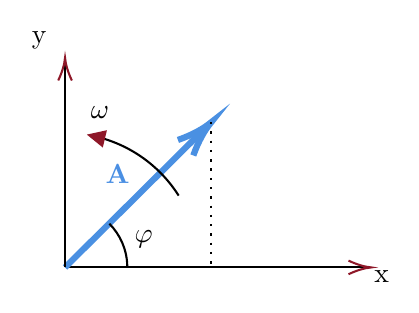
\begin{tikzpicture}[x=0.75pt,y=0.75pt,yscale=-1,xscale=1]
%uncomment if require: \path (0,15225); %set diagram left start at 0, and has height of 15225

%Straight Lines [id:da5927370156317948] 
\draw    (220,933) -- (365.5,933) ;
\draw [shift={(367.5,933)}, rotate = 180] [color={wsdred}  ][line width=0.75]    (10.93,-3.29) .. controls (6.95,-1.4) and (3.31,-0.3) .. (0,0) .. controls (3.31,0.3) and (6.95,1.4) .. (10.93,3.29)   ;
%Straight Lines [id:da34962116656860287] 
\draw [color={rgb, 255:red, 74; green, 144; blue, 226 }  ,draw opacity=1 ][line width=2.25]    (220,933) -- (287.66,865.82) ;
\draw [shift={(290.5,863)}, rotate = 135.2] [color={rgb, 255:red, 74; green, 144; blue, 226 }  ,draw opacity=1 ][line width=2.25]    (17.49,-5.26) .. controls (11.12,-2.23) and (5.29,-0.48) .. (0,0) .. controls (5.29,0.48) and (11.12,2.23) .. (17.49,5.26)   ;
%Shape: Arc [id:dp021810946519202234] 
\draw  [draw opacity=0] (241.38,911.96) .. controls (246.57,917.22) and (249.82,924.39) .. (249.99,932.32) -- (220,933) -- cycle ; \draw   (241.38,911.96) .. controls (246.57,917.22) and (249.82,924.39) .. (249.99,932.32) ;  
%Shape: Arc [id:dp8513799267562083] 
\draw  [draw opacity=0] (238,870.79) .. controls (253.36,875.22) and (266.37,885.19) .. (274.73,898.39) -- (220,933) -- cycle ; \draw   (238,870.79) .. controls (253.36,875.22) and (266.37,885.19) .. (274.73,898.39) ;  
%Straight Lines [id:da8048233056164524] 
\draw    (238,870.79) -- (233.42,869.69) ;
\draw [shift={(230.5,869)}, rotate = 13.39] [fill={wsdred}  ][line width=0.08]  [draw opacity=0] (8.93,-4.29) -- (0,0) -- (8.93,4.29) -- cycle    ;
%Straight Lines [id:da8962545520745455] 
\draw    (220,933) -- (220,834) ;
\draw [shift={(220,832)}, rotate = 90] [color={wsdred}] [line width=0.75]    (10.93,-3.29) .. controls (6.95,-1.4) and (3.31,-0.3) .. (0,0) .. controls (3.31,0.3) and (6.95,1.4) .. (10.93,3.29)   ;
%Straight Lines [id:da4834893344127229] 
\draw  [dash pattern={on 0.84pt off 2.51pt}]  (290.5,863) -- (290.5,933) ;

% Text Node
\draw (367.5,933) node [anchor=north west][inner sep=0.75pt]   [align=left] {x};
% Text Node
\draw (231,854) node [anchor=north west][inner sep=0.75pt]    {$\omega $};
% Text Node
\draw (252,914) node [anchor=north west][inner sep=0.75pt]    {$\varphi $};
% Text Node
\draw (238,882) node [anchor=north west][inner sep=0.75pt]   [align=left] {\textbf{\textcolor[rgb]{0.29,0.56,0.89}{A}}};
% Text Node
\draw (202.5,818) node [anchor=north west][inner sep=0.75pt]   [align=left] {y};


\end{tikzpicture}
    \caption{}
    \label{fig:1.10}
\end{figure}
Trên giản đồ, vector biểu diễn sự dao động của hệ sẽ xoay quanh gốc toạ độ với vận tốc góc \(\omega\), độ dài vector là \(A\). 
\vspace{2mm}

Nếu vật thể là tổng hợp của nhiều dao động điều hoà
\begin{equation*}
    x = x_1 + x_2 + x_3 + ... + x_n
\end{equation*}
Thì trên giản đồ, vector biểu diển cho \(x\) sẽ là tổng vector các thành phần dao động điều hoà.
\begin{figure}[!htb]
    \centering
    \definecolor{wsdred}{HTML}{8E1728}



\tikzset{every picture/.style={line width=0.75pt}} %set default line width to 0.75pt        

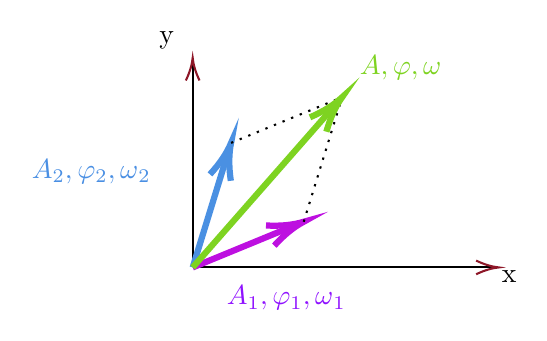
\begin{tikzpicture}[x=0.75pt,y=0.75pt,yscale=-1,xscale=1]
%uncomment if require: \path (0,15225); %set diagram left start at 0, and has height of 15225

%Straight Lines [id:da5927370156317948] 
\draw    (146,906) -- (291.5,906) ;
\draw [shift={(293.5,906)}, rotate = 180] [color={wsdred}  ][line width=0.75]    (10.93,-3.29) .. controls (6.95,-1.4) and (3.31,-0.3) .. (0,0) .. controls (3.31,0.3) and (6.95,1.4) .. (10.93,3.29)   ;
%Straight Lines [id:da34962116656860287] 
\draw [color={rgb, 255:red, 189; green, 16; blue, 224 }  ,draw opacity=1 ][line width=2.25]    (146,906) -- (195.8,885.52) ;
\draw [shift={(199.5,884)}, rotate = 157.65] [color={rgb, 255:red, 189; green, 16; blue, 224 }  ,draw opacity=1 ][line width=2.25]    (17.49,-5.26) .. controls (11.12,-2.23) and (5.29,-0.48) .. (0,0) .. controls (5.29,0.48) and (11.12,2.23) .. (17.49,5.26)   ;
%Straight Lines [id:da8962545520745455] 
\draw    (146,906) -- (146,807) ;
\draw [shift={(146,805)}, rotate = 90] [color={wsdred}  ][line width=0.75]    (10.93,-3.29) .. controls (6.95,-1.4) and (3.31,-0.3) .. (0,0) .. controls (3.31,0.3) and (6.95,1.4) .. (10.93,3.29)   ;
%Straight Lines [id:da9101145846792975] 
\draw [color={rgb, 255:red, 74; green, 144; blue, 226 }  ,draw opacity=1 ][line width=2.25]    (146,906) -- (163.32,849.82) ;
\draw [shift={(164.5,846)}, rotate = 107.14] [color={rgb, 255:red, 74; green, 144; blue, 226 }  ,draw opacity=1 ][line width=2.25]    (17.49,-5.26) .. controls (11.12,-2.23) and (5.29,-0.48) .. (0,0) .. controls (5.29,0.48) and (11.12,2.23) .. (17.49,5.26)   ;
%Straight Lines [id:da7014505903865442] 
\draw [color={rgb, 255:red, 0; green, 0; blue, 0 }  ,draw opacity=1 ][line width=0.75]  [dash pattern={on 0.84pt off 2.51pt}]  (199.5,884) -- (218,824) ;
%Straight Lines [id:da16436515246039618] 
\draw [color={rgb, 255:red, 0; green, 0; blue, 0 }  ,draw opacity=1 ][line width=0.75]  [dash pattern={on 0.84pt off 2.51pt}]  (164.5,846) -- (218,824) ;
%Straight Lines [id:da04823563439608747] 
\draw [color={rgb, 255:red, 126; green, 211; blue, 33 }  ,draw opacity=1 ][line width=2.25]    (146,906) -- (215.36,827.01) ;
\draw [shift={(218,824)}, rotate = 131.28] [color={rgb, 255:red, 126; green, 211; blue, 33 }  ,draw opacity=1 ][line width=2.25]    (17.49,-5.26) .. controls (11.12,-2.23) and (5.29,-0.48) .. (0,0) .. controls (5.29,0.48) and (11.12,2.23) .. (17.49,5.26)   ;

% Text Node
\draw (293.5,906) node [anchor=north west][inner sep=0.75pt]   [align=left] {x};
% Text Node
\draw (129,863) node [anchor=north west][inner sep=0.75pt]   [align=left] {};
% Text Node
\draw (128.5,791) node [anchor=north west][inner sep=0.75pt]   [align=left] {y};
% Text Node
\draw (67,852.5) node [anchor=north west][inner sep=0.75pt]    {$\textcolor[rgb]{0.29,0.56,0.89}{A}\textcolor[rgb]{0.29,0.56,0.89}{_{2}}\textcolor[rgb]{0.29,0.56,0.89}{,\varphi }\textcolor[rgb]{0.29,0.56,0.89}{_{2}}\textcolor[rgb]{0.29,0.56,0.89}{,\omega }\textcolor[rgb]{0.29,0.56,0.89}{_{2}}\textcolor[rgb]{0.29,0.56,0.89}{\ }$};
% Text Node
\draw (161,913.5) node [anchor=north west][inner sep=0.75pt]    {$\textcolor[rgb]{0.56,0.07,1}{A}\textcolor[rgb]{0.56,0.07,1}{_{1}}\textcolor[rgb]{0.56,0.07,1}{,\varphi }\textcolor[rgb]{0.56,0.07,1}{_{1}}\textcolor[rgb]{0.56,0.07,1}{,\omega }\textcolor[rgb]{0.56,0.07,1}{_{1}}$};
% Text Node
\draw (225,802.5) node [anchor=north west][inner sep=0.75pt]  [color={rgb, 255:red, 126; green, 211; blue, 33 }  ,opacity=1 ]  {$A,\varphi ,\omega $};

\end{tikzpicture}
    \caption{}
    \label{fig:1.11}
\end{figure}
\subsection{Toạ độ suy rộng (giới thiệu)}
\label{sec:1.5}
Trong các cơ hệ, biến của phương trình vi phân không nhất thiết là toạ độ dịch chuyển \(x\). Nó có thể là các đại lượng khác như 
\begin{equation*}
    \begin{array}{cl}
    \theta & \text{góc lệch} \\
    x_1 + x_2 & \text{tổng hợp các dao động thành phần (giống hình \ref{fig:1.11})} 
    \end{array}
\end{equation*}
Ta gọi chung các toạ độ suy rộng là \(q\). Nếu lúc đấy ta phương trình vi phân sau, thì ta vẫn nói hệ tuân theo quy luật dao động điều hoà.
\begin{equation}
    \ddot{q} + \omega^2 q = 0.
    \label{eq:1.20}
\end{equation}
**\textit{Tìm một ví dụ cho toạ độ suy rộng \(x_1 + x_2\) dao động điều hoà trong trường hợp của hình \ref{fig:1.11}.}

\section{Dao động hệ nhiều chất điểm liên kết}
Bây giờ hệ sẽ không chỉ gồm một chất điểm duy nhất dao động. Hệ có thể bao gồm 2, 3 hoặc nhiều chất điểm dao động hơn. Điểm khác biệt dễ thấy nhất là không chỉ có 1 phương trình động lực học, nhưng bây giờ sẽ là một hệ phương trình vi phân gồm n ẩn. 
\vspace{2mm}

Ta sẽ đi từ những ví dụ đơn giản, nơi mà chúng ta sẽ dùng trực quan toán học và vật lý để giải quyết. Sau đó, ta sẽ nói về các phương pháp dùng để giải quyết một các (tương đối) tổng quát.

\subsection{Hệ 2 chất điểm 3 lò xo}
\begin{figure}[!htb]
    \centering
    \definecolor{wsdred}{HTML}{8E1728}



% Pattern Info
 
\tikzset{
pattern size/.store in=\mcSize, 
pattern size = 5pt,
pattern thickness/.store in=\mcThickness, 
pattern thickness = 0.3pt,
pattern radius/.store in=\mcRadius, 
pattern radius = 1pt}
\makeatletter
\pgfutil@ifundefined{pgf@pattern@name@_gyar4beyw}{
\pgfdeclarepatternformonly[\mcThickness,\mcSize]{_gyar4beyw}
{\pgfqpoint{0pt}{0pt}}
{\pgfpoint{\mcSize+\mcThickness}{\mcSize+\mcThickness}}
{\pgfpoint{\mcSize}{\mcSize}}
{
\pgfsetcolor{\tikz@pattern@color}
\pgfsetlinewidth{\mcThickness}
\pgfpathmoveto{\pgfqpoint{0pt}{0pt}}
\pgfpathlineto{\pgfpoint{\mcSize+\mcThickness}{\mcSize+\mcThickness}}
\pgfusepath{stroke}
}}
\makeatother

% Pattern Info
 
\tikzset{
pattern size/.store in=\mcSize, 
pattern size = 5pt,
pattern thickness/.store in=\mcThickness, 
pattern thickness = 0.3pt,
pattern radius/.store in=\mcRadius, 
pattern radius = 1pt}
\makeatletter
\pgfutil@ifundefined{pgf@pattern@name@_hlwblp5cz}{
\pgfdeclarepatternformonly[\mcThickness,\mcSize]{_hlwblp5cz}
{\pgfqpoint{0pt}{0pt}}
{\pgfpoint{\mcSize+\mcThickness}{\mcSize+\mcThickness}}
{\pgfpoint{\mcSize}{\mcSize}}
{
\pgfsetcolor{\tikz@pattern@color}
\pgfsetlinewidth{\mcThickness}
\pgfpathmoveto{\pgfqpoint{0pt}{0pt}}
\pgfpathlineto{\pgfpoint{\mcSize+\mcThickness}{\mcSize+\mcThickness}}
\pgfusepath{stroke}
}}
\makeatother
\tikzset{every picture/.style={line width=0.75pt}} %set default line width to 0.75pt        

\begin{tikzpicture}[x=0.75pt,y=0.75pt,yscale=-1,xscale=1]
%uncomment if require: \path (0,15225); %set diagram left start at 0, and has height of 15225

%Straight Lines [id:da3223058949903339] 
\draw [color={rgb, 255:red, 0; green, 0; blue, 0 }  ,draw opacity=1 ]   (446.5,1088.22) -- (86,1088.22) ;
%Shape: Rectangle [id:dp7648671038082127] 
\draw  [draw opacity=0][pattern=_gyar4beyw,pattern size=6pt,pattern thickness=0.75pt,pattern radius=0pt, pattern color={rgb, 255:red, 0; green, 0; blue, 0}] (86,1047) -- (60.5,1047) -- (60.5,1088.22) -- (86,1088.22) -- cycle ;
%Shape: Resistor [id:dp6479321963022213] 
\draw  [color={rgb, 255:red, 0; green, 0; blue, 0 }  ,draw opacity=1 ] (86,1067.61) -- (102.65,1067.61) -- (106.35,1058.73) -- (113.75,1076.48) -- (121.15,1058.73) -- (128.55,1076.48) -- (135.95,1058.73) -- (143.35,1076.48) -- (150.75,1058.73) -- (158.15,1076.48) -- (161.85,1067.61) -- (178.5,1067.61) ;
%Shape: Square [id:dp15263822722006148] 
\draw  [color={rgb, 255:red, 0; green, 0; blue, 0 }  ,draw opacity=1 ] (178.5,1047) -- (219.72,1047) -- (219.72,1088.22) -- (178.5,1088.22) -- cycle ;
%Shape: Resistor [id:dp3406372469944945] 
\draw  [color={rgb, 255:red, 0; green, 0; blue, 0 }  ,draw opacity=1 ] (220,1067.61) -- (236.65,1067.61) -- (240.35,1058.73) -- (247.75,1076.48) -- (255.15,1058.73) -- (262.55,1076.48) -- (269.95,1058.73) -- (277.35,1076.48) -- (284.75,1058.73) -- (292.15,1076.48) -- (295.85,1067.61) -- (312.5,1067.61) ;
%Shape: Square [id:dp8671738733511334] 
\draw  [color={rgb, 255:red, 0; green, 0; blue, 0 }  ,draw opacity=1 ] (312.5,1047) -- (353.72,1047) -- (353.72,1088.22) -- (312.5,1088.22) -- cycle ;
%Shape: Resistor [id:dp4210341004898319] 
\draw  [color={rgb, 255:red, 0; green, 0; blue, 0 }  ,draw opacity=1 ] (354,1067.61) -- (370.65,1067.61) -- (374.35,1058.73) -- (381.75,1076.48) -- (389.15,1058.73) -- (396.55,1076.48) -- (403.95,1058.73) -- (411.35,1076.48) -- (418.75,1058.73) -- (426.15,1076.48) -- (429.85,1067.61) -- (446.5,1067.61) ;
%Straight Lines [id:da6091760378667466] 
\draw [color={rgb, 255:red, 0; green, 0; blue, 0 }  ,draw opacity=1 ]   (86,1047) -- (86,1088.22) ;
%Straight Lines [id:da1853906688587692] 
\draw [color={rgb, 255:red, 0; green, 0; blue, 0 }  ,draw opacity=1 ]   (446.5,1047) -- (446.5,1088.22) ;
%Shape: Rectangle [id:dp9695945528994532] 
\draw  [draw opacity=0][pattern=_hlwblp5cz,pattern size=6pt,pattern thickness=0.75pt,pattern radius=0pt, pattern color={rgb, 255:red, 0; green, 0; blue, 0}] (472,1047) -- (446.5,1047) -- (446.5,1088.22) -- (472,1088.22) -- cycle ;
%Straight Lines [id:da6417307585486507] 
\draw [color={rgb, 255:red, 0; green, 0; blue, 0 }  ,draw opacity=1 ]   (201,1118) -- (238.5,1118) ;
\draw [shift={(240.5,1118)}, rotate = 180] [color={rgb, 255:red, 0; green, 0; blue, 0 }  ,draw opacity=1 ][line width=0.75]    (10.93,-3.29) .. controls (6.95,-1.4) and (3.31,-0.3) .. (0,0) .. controls (3.31,0.3) and (6.95,1.4) .. (10.93,3.29)   ;
\draw [shift={(201,1118)}, rotate = 180] [color={rgb, 255:red, 0; green, 0; blue, 0 }  ,draw opacity=1 ][line width=0.75]    (0,5.59) -- (0,-5.59)   ;
%Straight Lines [id:da15068921372551158] 
\draw [color={rgb, 255:red, 0; green, 0; blue, 0 }  ,draw opacity=1 ]   (332,1118) -- (369.5,1118) ;
\draw [shift={(371.5,1118)}, rotate = 180] [color={rgb, 255:red, 0; green, 0; blue, 0 }  ,draw opacity=1 ][line width=0.75]    (10.93,-3.29) .. controls (6.95,-1.4) and (3.31,-0.3) .. (0,0) .. controls (3.31,0.3) and (6.95,1.4) .. (10.93,3.29)   ;
\draw [shift={(332,1118)}, rotate = 180] [color={rgb, 255:red, 0; green, 0; blue, 0 }  ,draw opacity=1 ][line width=0.75]    (0,5.59) -- (0,-5.59)   ;

% Text Node
\draw (127,1032.22) node [anchor=north west][inner sep=0.75pt]   [align=left] {$\displaystyle k_{1}$};
% Text Node
\draw (199.11,1067.61) node   [align=left] {$\displaystyle m_{1}$};
% Text Node
\draw (333.11,1067.61) node   [align=left] {$\displaystyle m_{2}$};
% Text Node
\draw (201,1123) node [anchor=north west][inner sep=0.75pt]    {$x_{1}$};
% Text Node
\draw (332,1123) node [anchor=north west][inner sep=0.75pt]    {$x_{2}$};
% Text Node
\draw (258,1032.22) node [anchor=north west][inner sep=0.75pt]   [align=left] {$\displaystyle k_{2}$};
% Text Node
\draw (390,1032.22) node [anchor=north west][inner sep=0.75pt]   [align=left] {$\displaystyle k_{3}$};


\end{tikzpicture}
    \caption{}
    \label{fig:2.1}
\end{figure}

Trong hệ này ta có các khối lượng \(m_1, m_2\) được liên kết với nhau bằng lò xo \(k_2\). Coi như hệ lý tưởng và tại vị trí như hình \ref{fig:2.1} các lo xò đang ở trạng thái tự nhiên. Ta xét trường hợp cơ bản với các giả thiết sau: \(m_1 = m_2 = m\), \(k_1 = k_3\). 
\vspace{2mm}

Phương trình động lực học cho từng chất điểm là
\begin{equation*}
    \begin{array}{ccc}
        m_1: & m \ddot{x}_1 &= - k_1 x_1 + k_2 (x_2 - x_1) \\
        m_2: & m \ddot{x}_2 &= - k_3 x_2 - k_2 (x_2 - x_1)
    \end{array}
\end{equation*}
Để giải quyết phương trình này, ta lần lượt cộng 2 phương trình; trừ 2 phương trình với nhau.
\begin{equation}
    \left\{
    \begin{array}{ccc}
    m ( \ddot{x}_1 + \ddot{x}_2) &=& - k_1 (x_1 + x_2).   \\
    m ( \ddot{x}_1 - \ddot{x}_2) &=& - (k_1 +2 k_2) (x_1 +x_2).
    \end{array}
    \right.
    \label{eq:2.1}
\end{equation}
Như mục \ref{sec:1.5}, ta đặt \(q_1 = x_1 + x_2\) và \(q_2 = x_1 - x_2\). Ta sẽ có hệ phương trình.
\begin{equation}
    \left\{
    \begin{array}{ccl}
    \ddot{q}_1 + \omega_1^2 q_1 &= 0 & \ , \text{với} \ \omega_1^2 = k_1/m \\
    \ddot{q}_2 + \omega_2^2 q_2 &= 0 & \ , \text{với} \ \omega_2^2 = (k_1+2k_2)/m
    \end{array}
    \right.
    \label{eq:2.2}
\end{equation}
Sau đấy ta có hệ phương trình
\begin{equation}
    \left\{ 
    \begin{array}{ccc}
    q_1 = x_1 + x_2 &=& A \cos{\left( \omega_1 t + \varphi_1\right)} \\
    q_2 = x_1 - x_2 &=& B \cos{\left( \omega_2 t + \varphi_2 \right)}
    \end{array}
    \right.
    \label{eq:2.3}
\end{equation}
Tương đương
\begin{equation}
    \left\{ 
    \begin{array}{ccc}
    x_1 &=& \frac12 \left(A \cos{\left( \omega_1 t + \varphi_1\right)} + B \cos{\left( \omega_2 t + \varphi_2 \right)} \right) \\
    \\
    x_2 &=& \frac12 \left(A \cos{\left( \omega_1 t + \varphi_1\right)} - B \cos{\left( \omega_2 t + \varphi_2 \right)} \right)
    \end{array}
    \right.
\end{equation}
Nhận xét: ở đây ta có thể thấy rằng toạ độ \(x_1\) là tổng hợp của hai dao động điều hoà \(q_1, q_2\) (tương tự với \(x_2\)). 

\subsection{Toạ độ trực giao}
Chúng ta đã giải quyết bài toán dao động liên kết ở trên bằng một số mẹo toán học. Ta nhận thấy rằng, nếu chỉ xét riêng toạ độ \(x_1\) hoặc \(x_2\) thì hệ sẽ không tạo nên một dao động điều hoà cơ bản. Nhưng nếu ta sử dụng toạ độ suy rộng \(q_1, q_2\) thì ta lại có thể giải quyết được. Người ta gọi các toạ độ thoả tính chất giống \(q_1, q_2\) là các toạ độ trực giao trong dao động liên kết. 
\vspace{2mm}

Các toạ độ trực giao sẽ khiến phương trình vi phân trở thành dạng như phương trình \ref{eq:1.20}. 
\end{document}
